\documentclass[11pt,nswissgerman]{article}
\usepackage{helvet}
\renewcommand{\familydefault}{\sfdefault}
\usepackage[latin2]{inputenc}
\usepackage[a4paper]{geometry}
\geometry{verbose,tmargin=3cm,bmargin=3cm,lmargin=3.5cm,rmargin=3.5cm,headheight=3cm,headsep=1cm,footskip=2cm}
\usepackage{fancyhdr}
\pagestyle{fancy}
\usepackage{wrapfig}
\usepackage{graphicx}
\usepackage[position=bottom]{subfig}
\usepackage{titletoc}
\usepackage{float}
\makeatletter
\@ifundefined{date}{}{\date{}}
\makeatother
\usepackage{babel}
\usepackage[
            colorlinks=true,
            urlcolor=green,
            linkcolor=black
]{hyperref}
\setcounter{secnumdepth}{1} % levels under \section are not numbered
\setcounter{tocdepth}{2}    % levels under \subsection are not listed in the TOC
\begin{document}
\author{Chantal Frunz}
\title{\Huge Erste Grosse Reise Korsika 2011\vspace{2cm}

\includegraphics[width=0.4\textwidth]{../Bilder/Logo/Logo.png}
}
\maketitle
\vfill
\tableofcontents

\newpage

\lhead{Korsika 2011 }

\rhead{jackthebus.com}

\cfoot{\thepage}
\subsection{03.09.2011 Samstag}
\begin{wrapfigure}{R}{0.45\textwidth} 
  \begin{centering}
    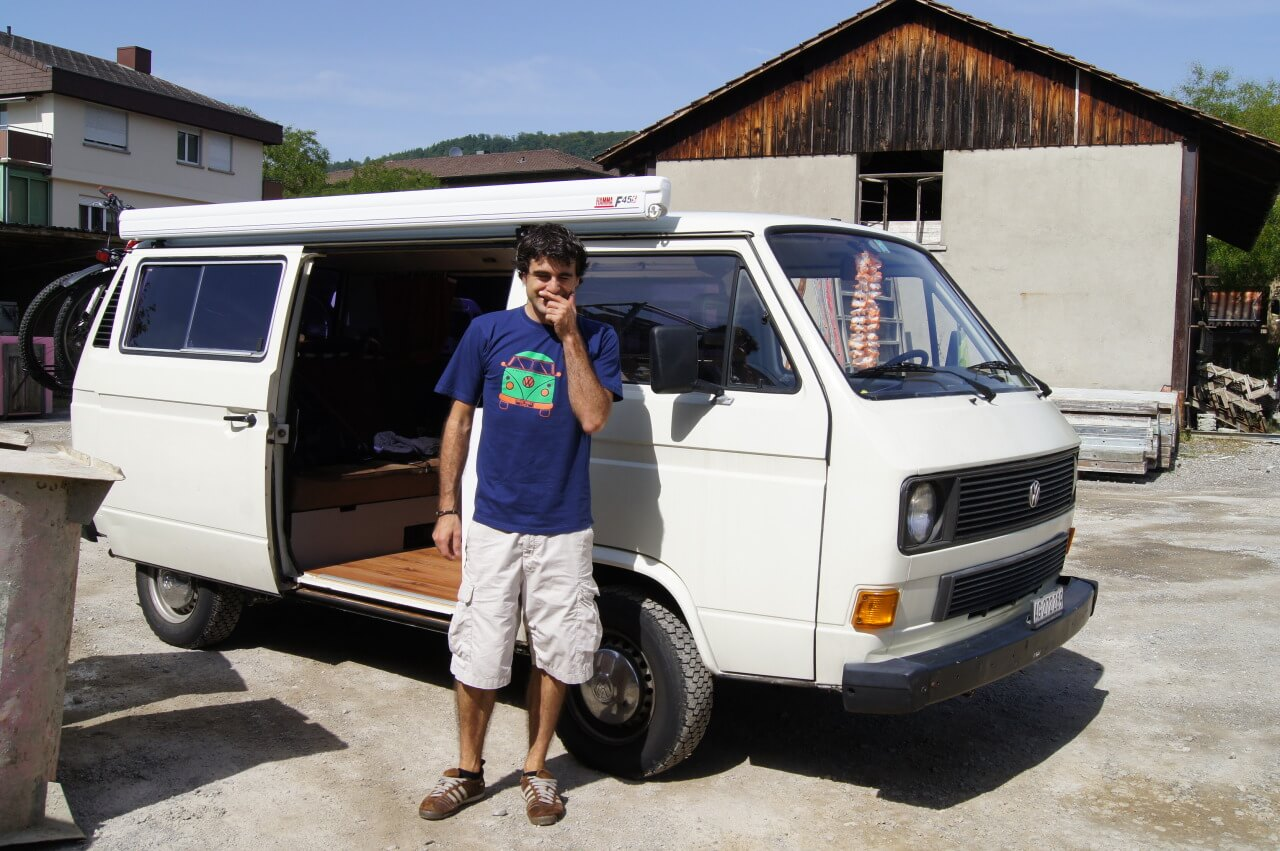
\includegraphics[width=0.4\textwidth, height=5cm, keepaspectratio]{../Bilder/Korsika/1.jpg}
    \caption{Uf gohts}
  \end{centering}
\end{wrapfigure} 
Morgenstund hat Gold im Mund... oder  au ned ;-) Am halbi 10ni simer �pe ufgstande und hend zersch mal gm�etlich zm�rgelet.
Da de Jack und de Philipp sehr gm�etlichi send, hends mer ja au chli chillig ch�ne neh;-) Scho am halbi 3 semer de startklar gsi und hend euse Jack vollglade...juhuuu, eusi erscht gross Reis met em B�sli cha afo! En Weggis hemer scho de erscht Stopp igleit und send chli an See gh�klet und hend �pis gesse und trunke.
Esch supersch�n gsi und sWetter esch traumhaft gsi.
Nach Weggis ha ich de mini Fahrk�nst welle zeige und be uf de Achsestross umed�sed...alli hend seeehr Freud a mer gha, well ich nat�rli en Speedy Consalez gsi ben:P
Vorem Gotthard, wos echli stockend witergange esch, send mini Nerve scho am Endi gsi und de Herr Bopp het m�esse witerfahre.
Mer send dor de Gotthard d�sed Richtig Italia...und sWetter esch emmer besser worde...chum send mer es Tessin cho hets afo seiche; dasch eus zemli bekannt vorcho.
E de erschte Rastst�tt em Tessin hets zNacht ge und zwar zwoi sehr chlini Portione Lasagne und Tortellini.
Meteme volle Mage und eme halbe Swimmingpool e eusem B�sli hemer die italienisch Grenze souver�n �berquert.
Zemli lang semer uf donkle, met Grillesound umgebni Strasse umekurvt bes mer denn dAutobahn gfonde hend.
Um di 10ni hemer de gfonde mer send f�r h�t gnueg uemd�st und send e Stond vor Genua ufe Rastst�tt go �bernachte.
Ruckzuckzackzack hemer euses Bettli parat gha und hend eus ed Decki ch�ne imulme.
dNacht esch echli unruhig gsi, neb de velle Autos wo cho und gange send, hend es paar obercooli Gangster gmeint sie m�sset ihri Mega-Boom-Boom-Musig en aller Lutst�rki eus abspele. 

\subsection{04.09.2011 Sonntag}
\begin{wrapfigure}{L}{0.45\textwidth} 
  \begin{centering}
    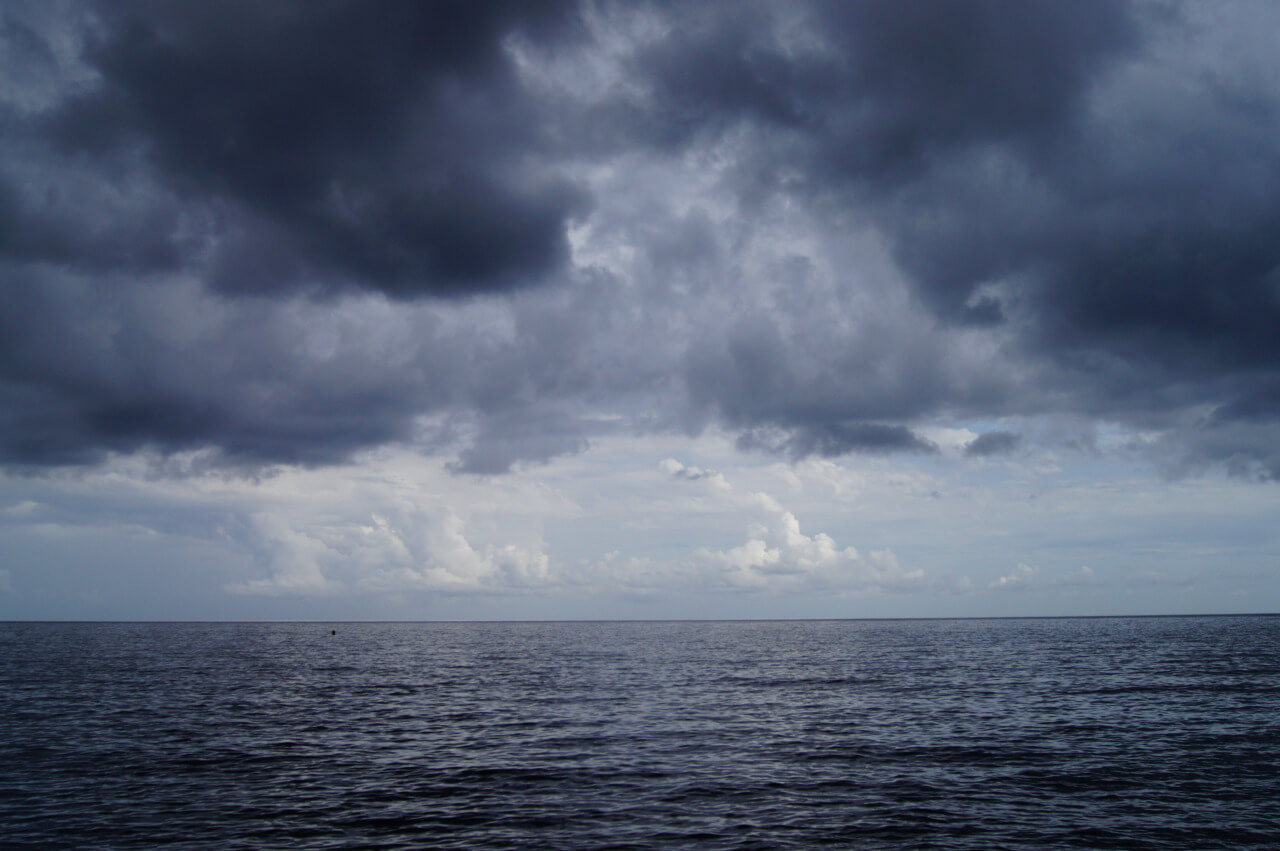
\includegraphics[width=0.4\textwidth, height=5cm, keepaspectratio]{../Bilder/Korsika/3.jpg}
    \caption{Nasser Empfang}
  \end{centering}
\end{wrapfigure} 
H�t esch fertig gsi met der Gem�tlichkeit...
versuchs mal mit Gem�tlichkeit, mit Ruhe und Gem�tlichkeit ;) scho am halb 6i semer ufgstande, hend gschnell zm�rgelet und send de schnell uf Genua d�set.
De Steff und de Jack het freud gha de kurveriche Autobahn.
Ich ha schochli Angst gha, dass mer eusi F�hri verpasset, well ufem Ticket staht, dass mer 90min vor Abfahrt scho muess ischiffe...
aber mer send p�nktlich, vellecht fasch zu p�nkltich f�r Italiener, be euse Moby Wonder acho und setzted jetzt grad ufem Deck und gn�ssed die sch�n Ussecht und dRegetr�pfli und de Wind ;) Aber siehe da dSonne esch de doch na v�recho und mer hend nachli ch�ne s�nnele e eusne Liegest�ehl.
Pl�tzlich hemer e chlini Insle und Elba ersp�ht und schlussendlich au Korsika...Korsika we are coming:) 
Met euse chline F�hri semer en Hafe vo Bastia man�vriert.
Trotz emene m�ehsame Alarmsignal esch alles guet gange und euse Jack esch gsond und ufem korsische Festland acho.
Mer send geg de Strom en Norde ufegfahre Richtig Cap Corse.
En Erbalunga hemer euse erscht Stopp gmacht und send dor die supersch�ne Altstadt bis zum Hafe gschlenderet.
Vo allem M�gliche hemer m�esse es F�teli mache ;)... alti gelb-orangi-toskanisch-aghuchti H�sli, romantischi engli G�ssli und vell herzigi Kaffis und Restaurants.
Aber leider hend eus dRegetr�pfli oder besser gseit riesigi Regetropfe bis nach Korsika verfolgt...wo mer am Hafe unde gsi send hets afo Tr�pfelet.
Gli hets afo Seiche und er send zum Jack zruggsecklet.
Denn eschs ersch recht losgange, de Petrus hets guet met eus gmeint, es esch emmer meh cho regne bis euse Jack eme Boot gliche het....
be mer hets sogar inegsprudlet!! Aber dor die superbreite und guet preparierte Strosse esch da ja ke Problem gsi.
Eigentli hemer welle en Macciagio �bernachte, aber da eusi Sicht ja biizli igschr�nkt gsi esch, hemer de Campingplatz verpasst.
Mer send tapfer witergfahre und send de ad Westk�ste cho...
ah ja da eschs Wetter ja vell besser gsi;) Jetzt semer au na fasch devogfloge! Aber damol hemer dAbzwigig f�r de Campingplatz en Centuri-Port ned verpasst und send das schmale Wegli bes zum Meer abekurvt.
De Campingplatz esch u herzig gsi, klein aber oho.
Mer hend eusi super Usr�stig met Store nat�rli ufbaut, send go dusche und hend eus uf de Weg nacheme Restaurant gmacht...
leider ned erfolgrich.
Dev�r hemer en wondersch�ne Sonneuntergang am Hafe unde ch�ne gn�sse.
Uf de Suechi nach Esse semer weder zo eusem Camping ufegloffe und damal hemer Gl�ck gha....
hmmm ufere chline Terrasse hemer fein gschlemmeret...
Entercote, Calamari, Frites und e Fl�sche Wii ;) Gschlafe hemer t���f und fescht, gw�ssi Persone send grad en Ohmacht gfalle;)

\begin{figure}[hb]
    \centering
    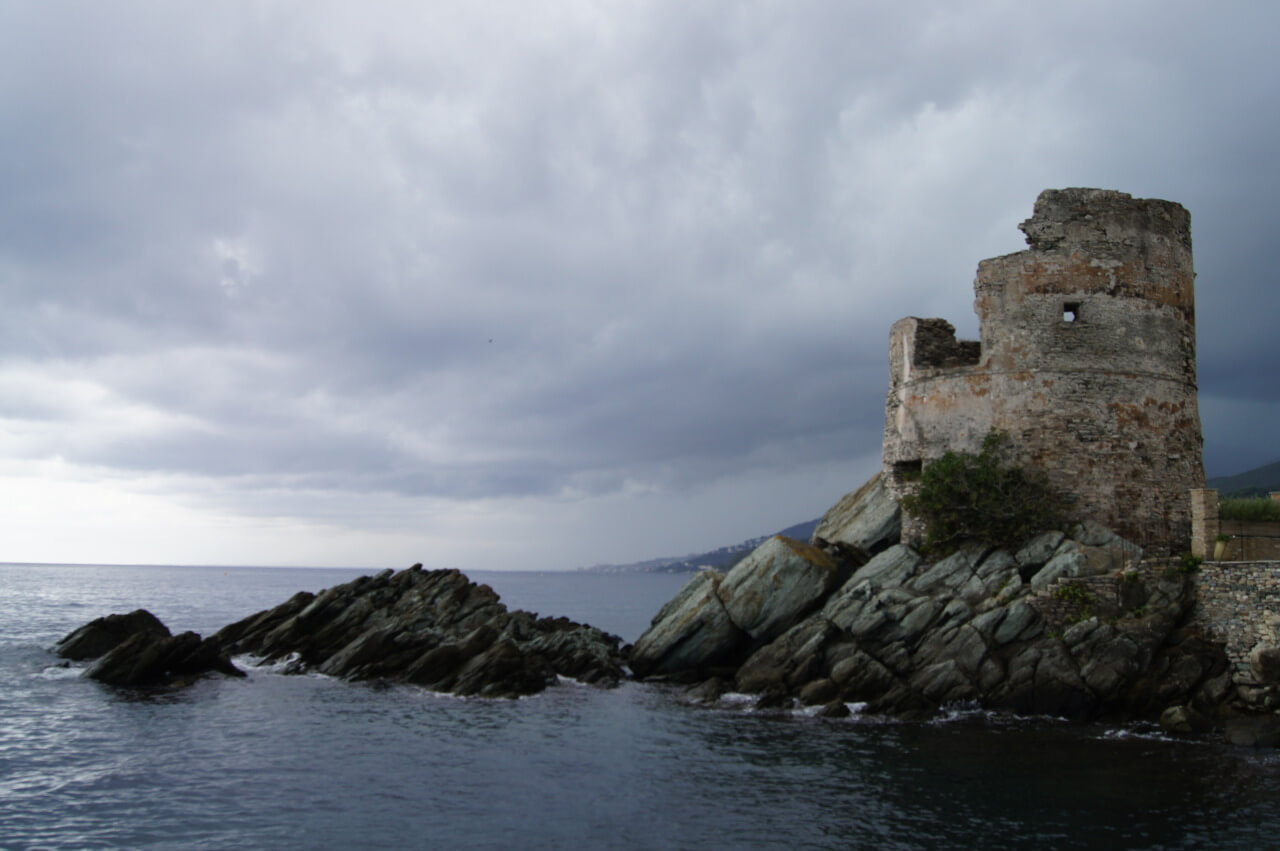
\includegraphics[width=\textwidth]{../Bilder/Korsika/4.jpg}
    \caption{Wetter het no Rum zur Verbesserig}
    \label{img:Korsika1}
\end{figure}

\pagebreak

\subsection{05.09.2011 Montag}

\begin{wrapfigure}{L}{0.45\textwidth} 
  \begin{centering}
    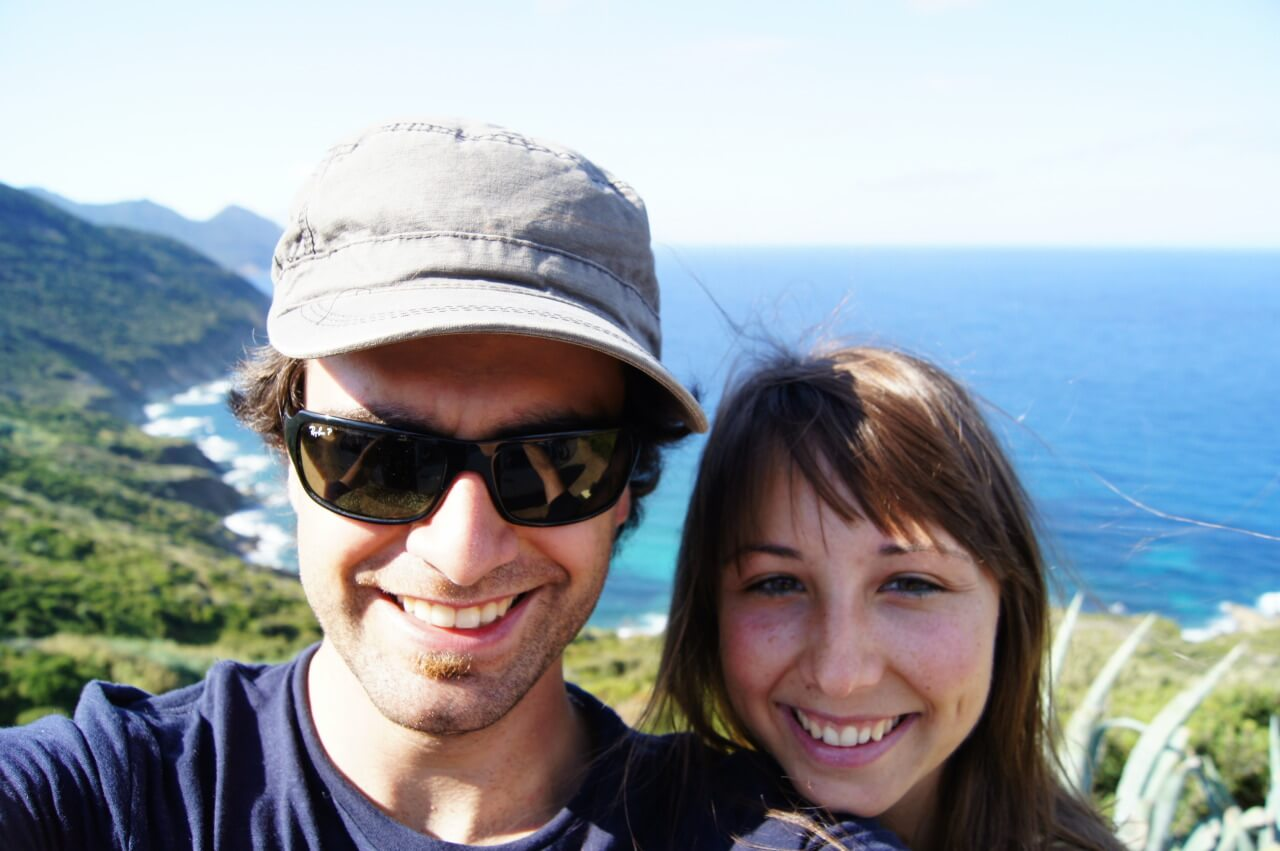
\includegraphics[width=0.4\textwidth, height=5cm, keepaspectratio]{../Bilder/Korsika/6.jpg}
    \caption{Zwei Entdecker uf Korsika}
  \end{centering}
\end{wrapfigure} 

\begin{figure}[b]
   \centering
      %\subfloat[CAPTION]{BILDERCODE}\qquad
   \subfloat{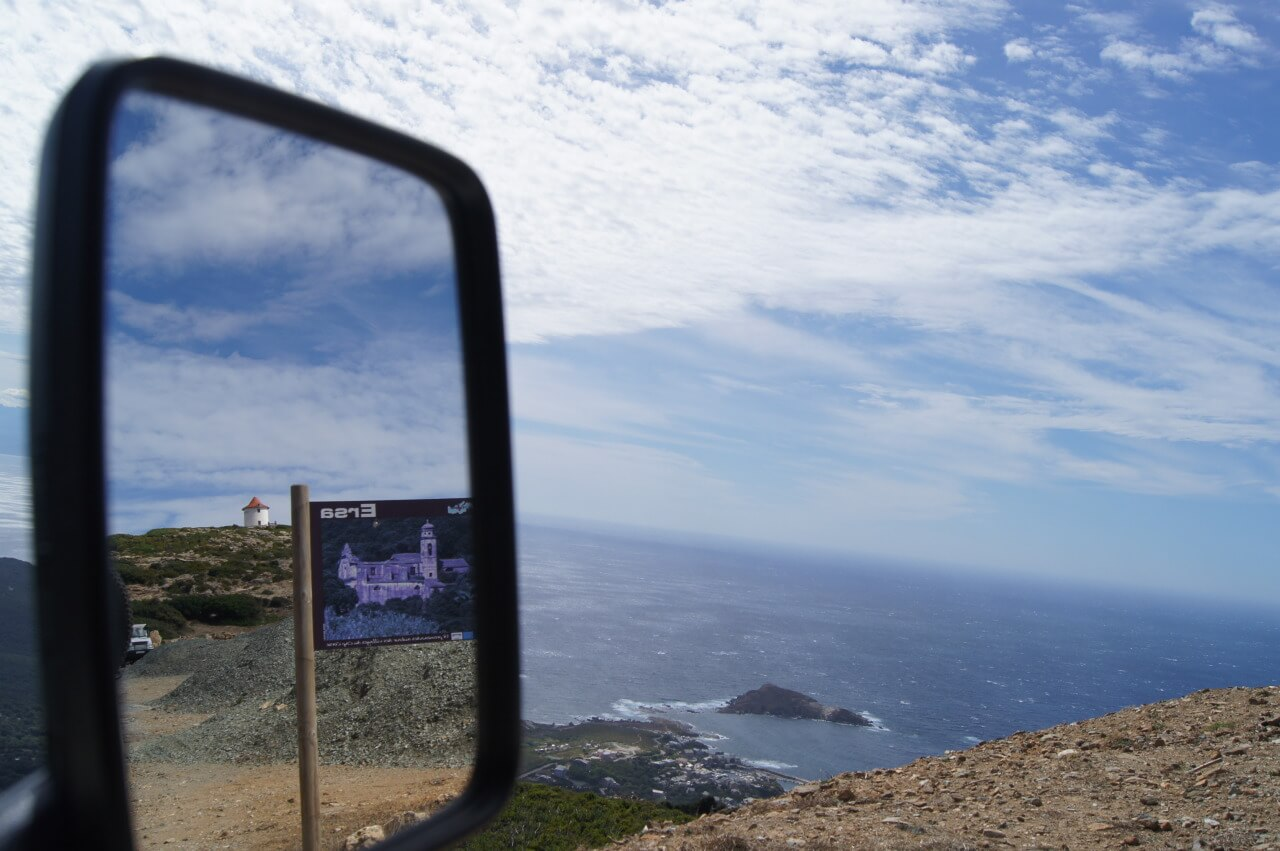
\includegraphics [width=0.3\textwidth]{../Bilder/Korsika/7.jpg}}\quad
   \subfloat{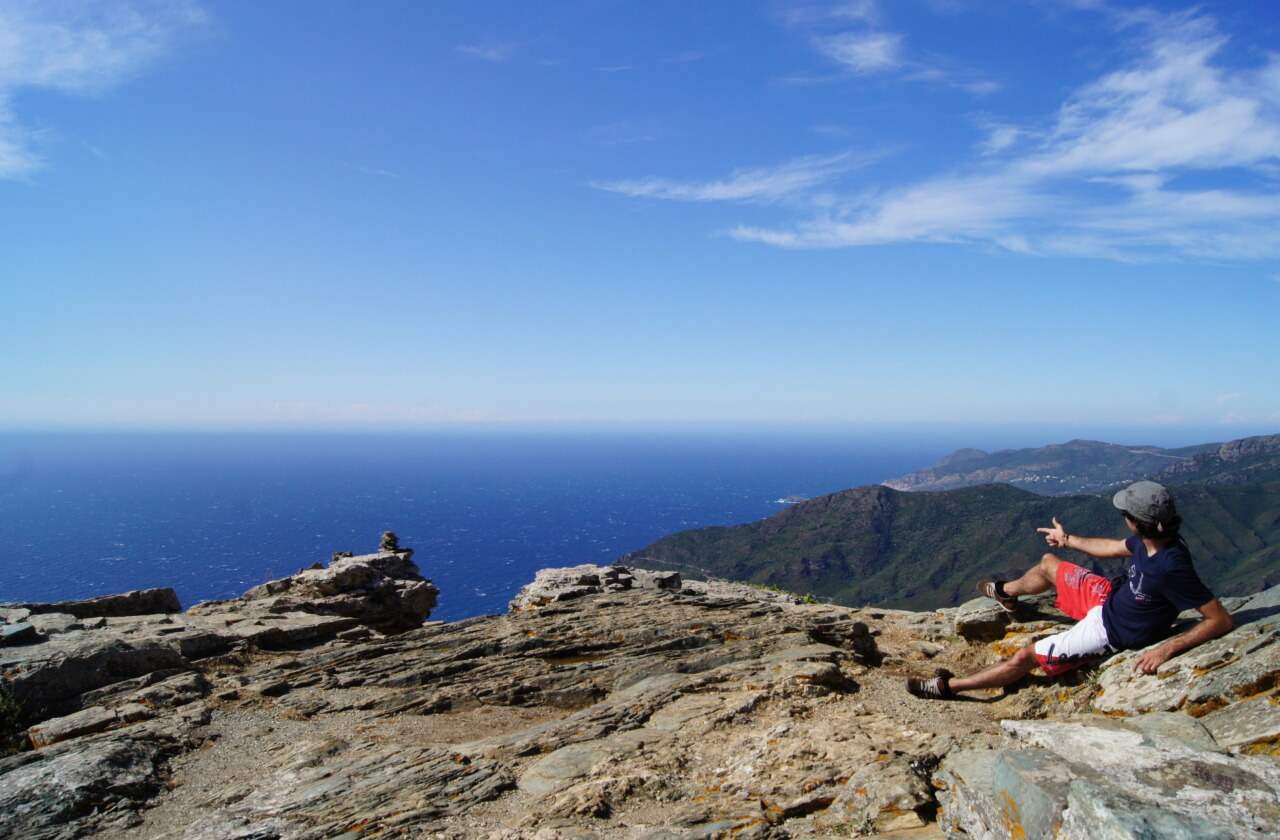
\includegraphics [width=0.3\textwidth]{../Bilder/Korsika/11.jpg}}\quad
   \subfloat{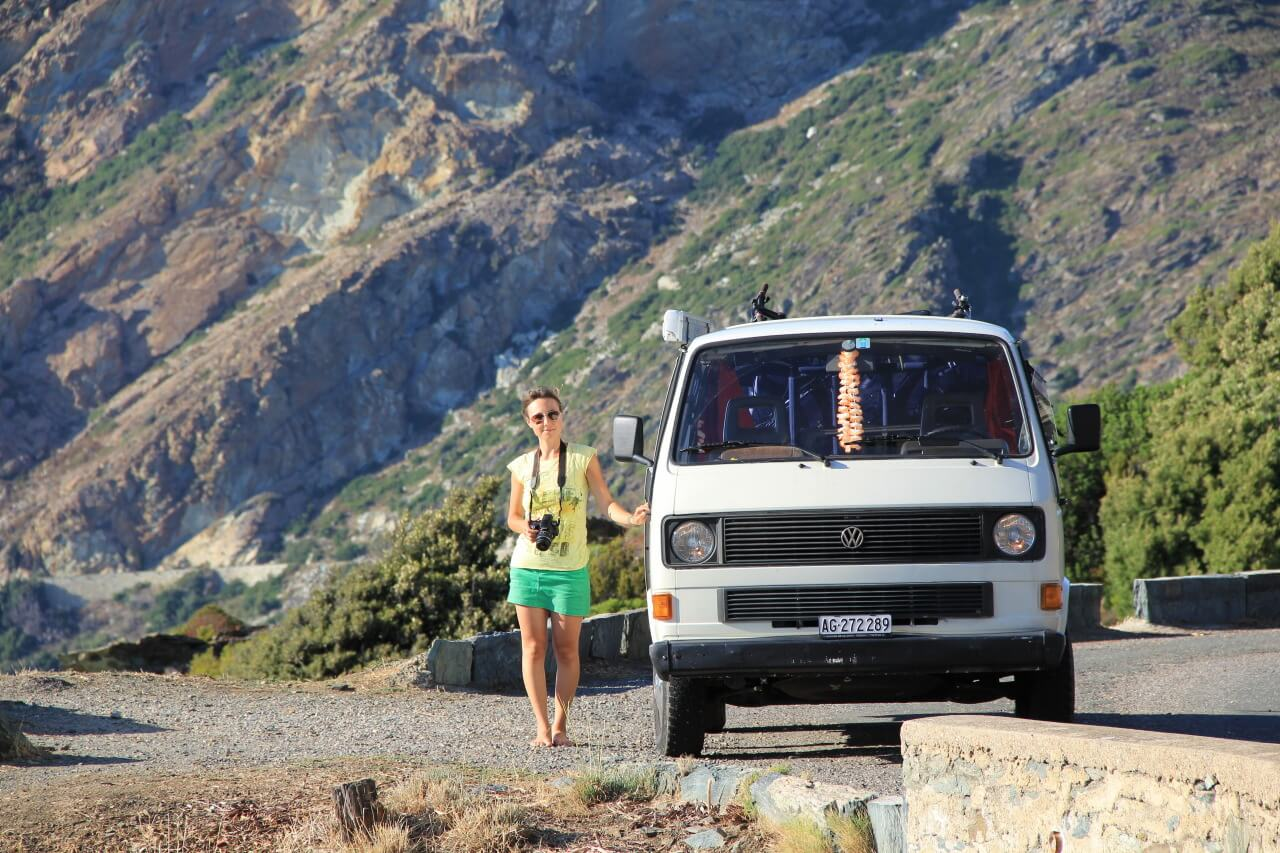
\includegraphics [width=0.3\textwidth]{../Bilder/Korsika/12.jpg}}\quad
   \caption[Korsika wie im Birlderbuech]{Korsika wie im Bilderbuech}
\end{figure}
Sonnen-Sonnen-Sonnenschein :-) In aller Frische und met eme chline Durscht semer um di 9ni ufgstande.
Zum zMorge hets suuuperfeini Croissant und en starke Kaffi ge.
Nach dem Kaffi hemer euses B�sli so schnell wie no nie ufgrumet gha und mer send back to the road an n�rdlichst Ponkt vo Korsika uf Barcaggio gfahre.
Vo Ersa het wedermal es sehr abent�rlichs Str�sslii ad K�ste gf�hrt.
De Jack und de Superdriver hend das aber super gmeisteret und mer send belohnt worde met ere wondersch�ne Bucht met de Insle Giraglia im Hintergund und emene ned allzu sch�ne Strand.
Jetzt hets gheisse: s�nnele, usruhe und vor allem B�dele...hihi...ich kenn da �per wo sich nachem B�dele gsehnt het und de nor bes zode Chn� es Wasser esch und de scho gnueg vom Bade gha het;) sWasser esch glasklar gsi und mer h�tt wit use ch�ne laufe.
Mer send de aber em Strand noche Richtig Genueseturm gloffe und hend na es chlises Restaurant gfonde, wo mer �pis trunke hend.
De semer au scho gli weder gange, well mer na es rechts Programm vor eus gha hend...nor hemer ned gw�sst das das au e Wanderig beinhaltet;) Mer send alles de K�ste entlang Richtig Pino gfahre und hend ufem Weg vell chlini herzigi Bergd�rfli atroffe.
En Pino send mer abboge f�r uf de Seneca-Ussechts-Turm.
Anstatt es winzigs Str�ssli wo mer erwartet hend, hets e sch�ni terreti Stross gha.
Scho vo witem hemer de Turm in weiter H�he obe gseh, aber dStross het de leider gar n�m so h�ch ufegf�hrt und mer hend m�esse zFuess witerga, obwohl de Turm emmer recht wit obe gsi esch.
Euse Wanderer het gmeint es g�ch 2 Stond und dOptimistin het met 30min grechnet..schlussendlich sends �pe 40 Minute gsi, wo mer steil de Berg hend m�esse ufeklettere.
Teilwis hemer w�rkli m�esse eusi Chletterk�nst uspacke und hend chli zwiflet, �b das w�rkli de rechtig Weg esch.
Dobe acho semer de met ere wooondersch�ne Ussecht belohnt worde.
dOst- und Westk�ste vom Cap Corse und die sch�n h�gelig Landschaft em Landesinnere hend mer ch�ne bestune.
Nat�rli ha ich grad es paar Panoramas m�esse sch�sse.
Nacheme usgibige Fotoshooting hemer de Abstig en Agriff gno und send de rechtig St.Florent d�set.
Nach Nonza hemer de euse Campingplatz A Stella gfonde.
Dummerwis semer ned grad direkt ad Rezeption gfahre, was dFrau Rezeptionistin alias Hilfsherif gar ned lostig gfonde het.
Sie het sich fasch n�m ch�ne erhole, het eus de aber doch na dErlaunis ge zum �bernachte.
Mer hend eus de au en super Platz direkt vorem Strand ade pole position gsicheret.
Es esch zwar chli schief gsi, aber mer hend e traumhafti Ussecht ufs wilde Meer gha.
De Sonneuntergang hemer met eme Campari und Chips uf eusne Ligist�he gnosse.
Zum Znacht hets Tomatesalat met Brot und Korsische Worscht ge.
Nachem Esse hend mer de Sternehimmel bestunt und jeglichi Sternschnuppe, Satellite und sogar Ufos ersp�ht;-) Nachem Sternegucke und Philosophiere send mer de meteme sch�ne (bizli lute) Wellerusche zfride ipfused.

\subsection{06.09.2011 Dienstag}
\begin{wrapfigure}{L}{0.45\textwidth} 
  \begin{centering}
    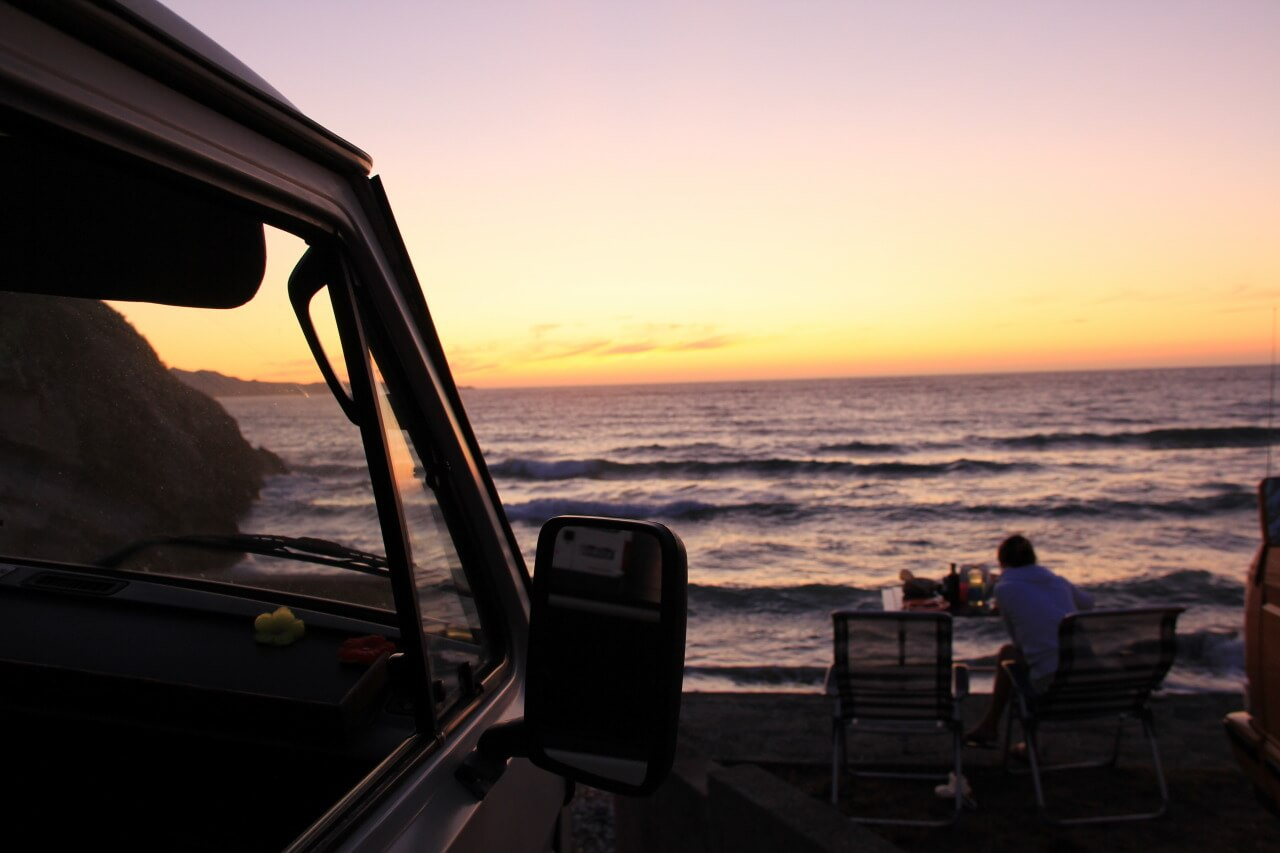
\includegraphics[width=0.4\textwidth, height=5cm, keepaspectratio]{../Bilder/Korsika/18.jpg}
    \caption{Zwei Entdecker uf Korsika}
  \end{centering}
\end{wrapfigure} 
Au ufgwacht semer metemene rusche... Wellerusche :) zM�rgelet hemer met ere geniale Ussecht uf die sch�n Bucht und send de au scho gli wederemal loszottlet.
A St.Florent semer verbigurket, well mer grad chli gschockt gsi send vo de velle L�t wos d�t gha het;) Witer Rihtig Ille Rousse hemer es paar wondersch�ni Str�nd gsichtet und send de be de vo Lozuri go b�dele.
Es het recht grossi Welle gha und de Steff het mer fasch n�m ch�ne usem Wasser bringe....ich be rechtig erstunt gsi und has chum ch�ne glaube.
Nach erschte skeptische An�cherige het er sich vode Welle n�me ch�ne trenne und esch am Strand em Welletakt ufe und abegrugelet....oh Wunder das er nacher e halbi Tonne Sand e sinere Hose gha het;-) Nachem B�dele und S�nnele semer de witer und hend en Ille Rousse en Stop gmacht.
WOW...die rote Granitfelse em t�rkisblaue Wasser hend eifach traumhaft usgseh! Mer hend en Spaziergang (met echli chlettere) zum Genuese- und L�chtturm gmacht, wo mer eifach en grandiosi Ussecht ufs St�dtli und die karibik�hnliche Buch gha hend.
Denn hemer en feini Crepes verschlunge und send nach Calvi gfahre.
Em grosse und sch�ne Campingplatz La Pinede hemer eus niederglo, hend eus fr�sch gmacht und send met em Velo ed Downtown Calvi gfahre.
Em Strand und de Isebahngleis nache semer d�set und hend en supersch�ni Ussecht uf Zitadelle vo Calvi gha.
Calvi esch en mega herzigi und touristischi Stadt met herzige G�ssli, L�deli, vellne Gelati-St�nd und sch�ne Restaurant am Hafe entlang.
Mer send enes Restaurant, wo em Reisef�hrer empfole worde esch und es esch eifach genial gsi...hmm de Steff het Teigware met Meeresfr�cht gha und ich Lachs met Ris und Gm�es. himmlisch:) Gl�cklich und met vollem Buch semer zom Camping zrugfahre und send go pfuuuse. 

\subsection{07.09.2011 Mittwoch}

sErscht mal hemer 2 N�cht uf eim Camping �bernachtet und so hemer en super gm�etliche Tag gmacht en Calvi.
Sch�n usgschlafe hemer, fein zm�rgelet und de semer met de Velos es Altst�dtli vo Calvi d�set.
Zersch semer go Zidatelle aluege, was zemli imposant gsi esch.
Neb de hoche Mure hets ganz vell sch�ni Sujets vo alte H�ser, Fenster und T�re gha zum Fotografiere, mer zwoi Hobbyfotografe hend n�m welle ufh�re met F�tele;) De Innehof vode Zidatelle esch na zemli gross gsi und es het so usgseh, wie na L�t e dene alte H�ser l�bet.
Die Zitadelle und die velle Genueset�rm send na Relikt vode genuesische Herrschaft, wo fasch es Jahrhundert �ber Korsika regiert hend.
Nach dem spannende Rundgang semer zrug zo eusem Camping hend eusi Bad- und Schnorchelsache ipackt und send an Strand.
D�t hemer gs�nnelet, b�delet und sogar gschnorchlet! Em Meer hesch mega wit use ch�ne laufe..
de Steff esch fasch de ganz Weg met de Flosse usegwatschlet;) Bem Schnorchle hemer paar sch�ni selbrigi Fisch gseh und de Steff het sogar en Tintefisch gseh, angeblich;) Ich ha n�t gseh, well de Steff so umegfuchtlet het, dass er mit sine Flosse en ganze Sandstorm veranstaltet het;) Nach dem astrengende Schnorchle semer zo eusem Jack zrug und hend fein zNacht kochet: Spaghetti met Carbonara-Sauce.
Korsische Wy hemer na kauft, aber leider esch de zemli sur gsi.
Es esch super gm�etlich gsi und mer hend gnueg Zyt gha zum die andere Camper (vor allem D�ne) met erne T�ff zbeobachte.

\begin{figure}[H]
    \centering
    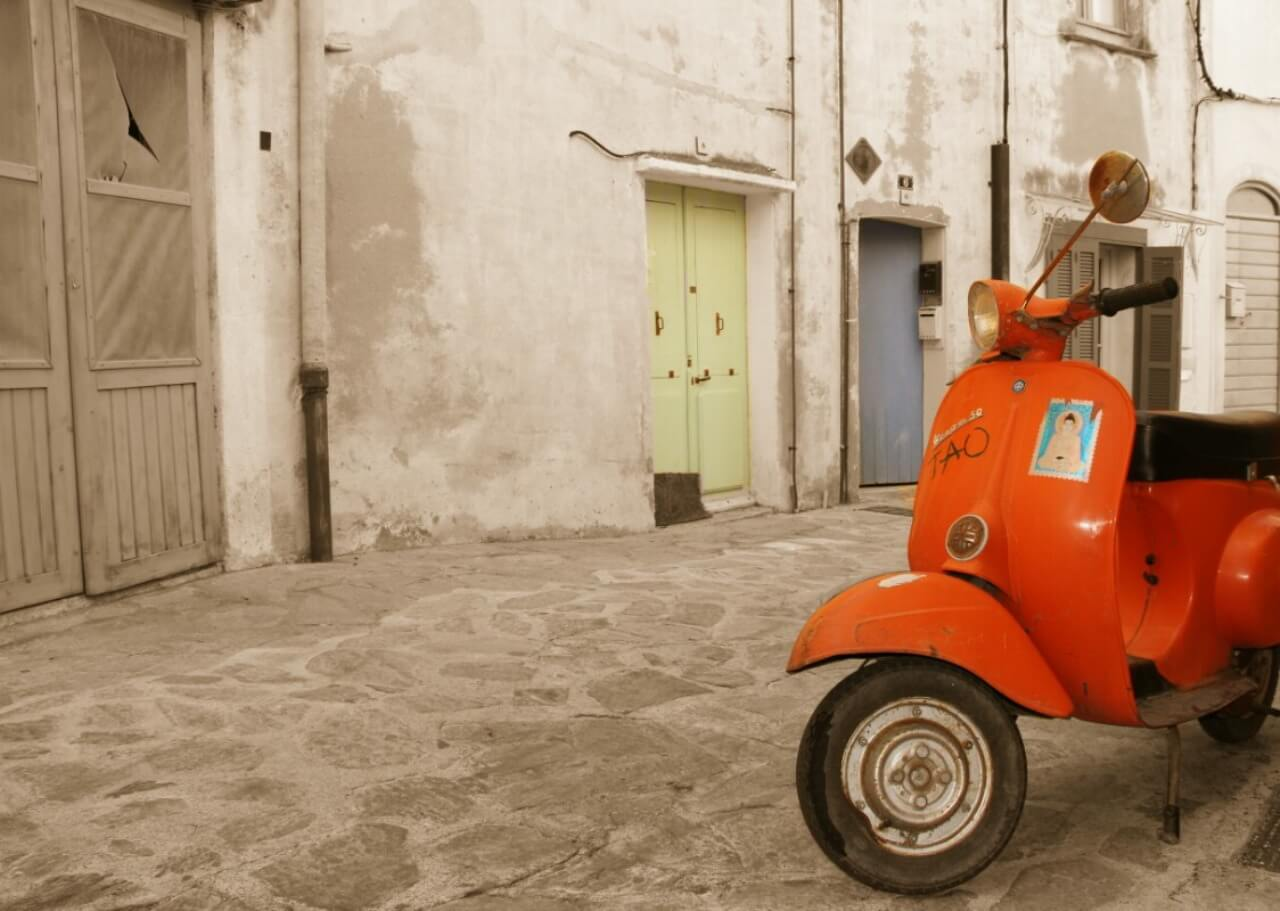
\includegraphics[width=\textwidth]{../Bilder/Korsika/25.jpg}
    \caption{Wunderbari G�ssli}
    \label{img:Korsika2}
\end{figure}
\pagebreak

\subsection{08.09.2011 Donnerstag}

\begin{wrapfigure}{L}{0.45\textwidth} 
  \begin{centering}
    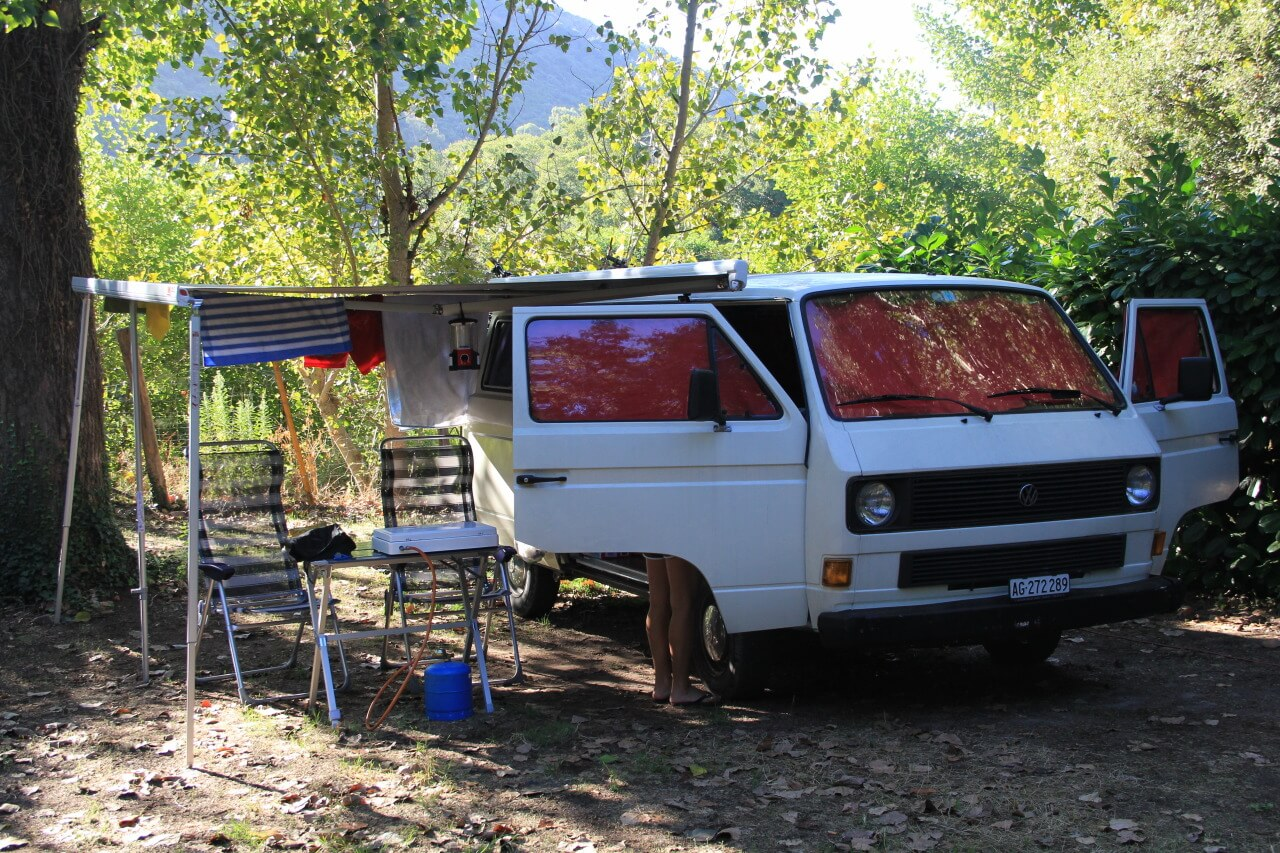
\includegraphics[width=0.4\textwidth, height=5cm, keepaspectratio]{../Bilder/Korsika/32.jpg}
    \caption{Jack in Action}
  \end{centering}
\end{wrapfigure} 

Scho am 8ti, so fr���e, semer ufgstande und hend eus los gmacht f�r en grossi Etappe.
Euses Ziel esch Porto gsi.
Ufem kurvige pass�hnliche Weg h�mer es mega sch�ns Resti anere Bucht gseh und hend denkt, d�t ch�mer sch�n zm�rgele.
Es esch au wodersch�n gsi, nor de Weg zo dem �rtli esch zemliii steinig gsi.
Aber de Jack het da super �berstande.
Met wondersch�ne Ussecht hemer en feine Kaffi gnosse.
Zrugg uf de Stross hemer witeri fantastischi Buchte erblickt und hend ufeme Ussechtsponk zm�rgelet.
Es het weder es paar F�teli ge..damol sogar na vo Libelle und Schmetterling..ah nei vo Schmetterling ned, well de Herr Bopp vo dere wilde Kreatur devogsecklet esch rings um de Jack..
hihi die andere Touriste hend zemli komisch glueget.
Aber au ich be a dem Tag unter schlechtem Insekte-Zeiche gstande.
Min Wespistech, wo ich mer am Obe vorane leider zuezoge ha het afo bisse und na dezue send mindestens 2 witeri Ficher bem Fahre es B�sli gfloge und ich ha fasch es Herzchriesi becho.
Darum be ich die ganz Fahrt zemli verchrampft em Auto ghocked.
Leider het sich au euse Superdriver chli m�esse verchrampfe, well ufem Weg nach Porto, zwoi riese Cars gmeint hend, sie m�sset die winzig schmale und kurvige K�stestr�ssli ne! So hets nat�rli en riese Stau ge und alli hend vorw�rts oder r�ckw�rts en Nischeplatz m�esse sueche.
Wo die superschlaue Cars verbi gsi send, hemer ch�ne witerfahre und send scho gli en Porto gsi.
De Golf vo Porto esch de sch�nst vo Korsika, aber leider daher au sehr touristisch.
dNatur esch wondersch�n met de knallrote Granitfelse (Em Oste hets vor allem Schiefer(Meeressedimeten)) und em t�fblaue-t�rkise Meer.
Mer send dors D�rfli spaziert, am Genueseturm verbi, well mer d�t h�t m�esse zahle und send an Kiesstrand gh�cklet.
D�t hemer leider ned ch�ne bade, well dWelle zu h�ch gsi send.
sGanze D�rfi esch eus vorcho wie em Europapark..ergendwie ned so atmosph�risch und eifach zemli k�nstlich.
Mer hend eus entschiede, gli weder ufzbreche und e chlini Wanderig em Calanche-Gebirge zmache.
Leider hets au d�t zemli vell L�t gha, aber die rot-orange Granitskulpture send schono idr�cklich gsi.
�pe e Stond em Ganze semer umegwaschlet und hend dFelsformatione, die steile Klippene und die wondersch�ne Buchte bestunt.
Denn es witer gange richtig Sagone.
Eigentli hemer en Porto welle �bernachte, aber die velle Bluemch�l-Touriste und de Weg zrug hend eus dra ghinderet.
Mer send de witer dere sch�ne, chli enge K�stestross entlang be Piana und Cargese verbi, bes nach Sargone.
D�t hemer en grosse sch�ne Camping gfonde met Restaurant, Swimming Pool und Tennisplatz....nor send mer fasch allei gsi;) Zum Znacht hemer Omelette gmacht met Banane, Zucker und Zitrone.
Es esch supi gsi...hihi...nor het �per chli welle pl�fe und het dOmelette ede Pfanne met Schwung m�esse chere...leider het sich de Henkel gl�st und die sch�n Omelette esch an Bode t�scht...da het �per sch�n dumm glueget;) Dev�r esch �per andersch vom Campari chli gflasht gsi und hets chli lostig gha;) Fig und Fertig semer es Bettli plumpst.

\pagebreak

\subsection{09.09.2011 Freitag}

\begin{wrapfigure}{R}{0.45\textwidth} 
  \begin{centering}
    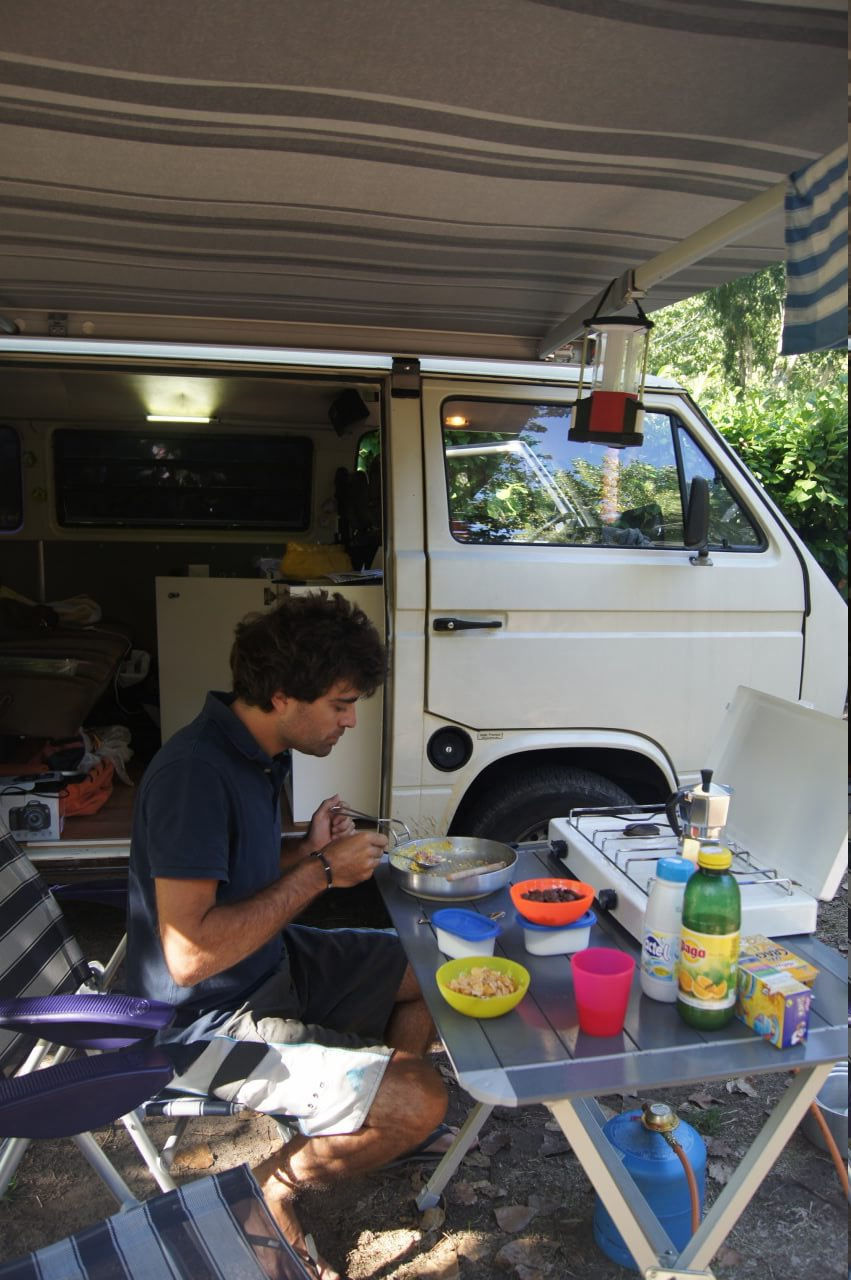
\includegraphics[width=0.4\textwidth, height=5cm, keepaspectratio]{../Bilder/Korsika/33.jpg}
    \caption{Zmorge}
  \end{centering}
\end{wrapfigure} 

H�t hemer feini M�esli und de Rescht vo eusere Omelette...R�ereier;) zum zMorge gha. 
Nachem zM�rgele hemer scho gli mal welle anen Strand go eus erhole vo de gestrige Strapaze.
En Liamone hemer en wondersch�ne Strand atroffe, wo S�ess- und Salzwasser z�mechond.
Schnell semer an Strand v�re und hend fasch n�me weg.
De Strand esch supersch�n gsi, sWasser glasklar und dWelle zemli gross.
De Pf�di het weder u Freud gha a dene Welle und esch rechtig go plantsche:) Mich hets au einisch sch�n am Strand nochezoge, was e sandigi Badhose met sich brocht het;) Speedminton hemer na versuecht zSpele, was be dem heftige Wind aber recht schwerig gsi esch.
Schliesslich hemer eus begn�egt met Fulenze, Lese und S�nnele...
die einte hends chli �bertrebe met de Sonne:-P Um di Dr� semer witer nach Propriano.
Weder �ber kurverichi Str�ssli semer de K�ste entlang und de witer es Landesinner bes nach Ajaccio.
Vo d�t het denn en grossi Strass nach Propriano gf�hrt, was allerdings ned heisst, dass sie ke Kurve het und ned ufe gat.
Jetzt semer emene herzige Camping direkt am Meer grad vor Propriano am Strand vo Calanca.
Nacheme sch�ne Sonneuntergang am Strand hemer fein zNacht (Tortellini, Gurkesalat) kochet und hend damal en bessere Wy ganz wegputzt...uiuiui..das w�r jetzt Stichwort gsi zum go pfuse;) Esch wedermal en supersch�ne Tag gsi..Hasta la vista:)

\subsection{10.09.2011 Samstag}
\begin{figure}[b]
   \centering
      %\subfloat[CAPTION]{BILDERCODE}\qquad
   \subfloat{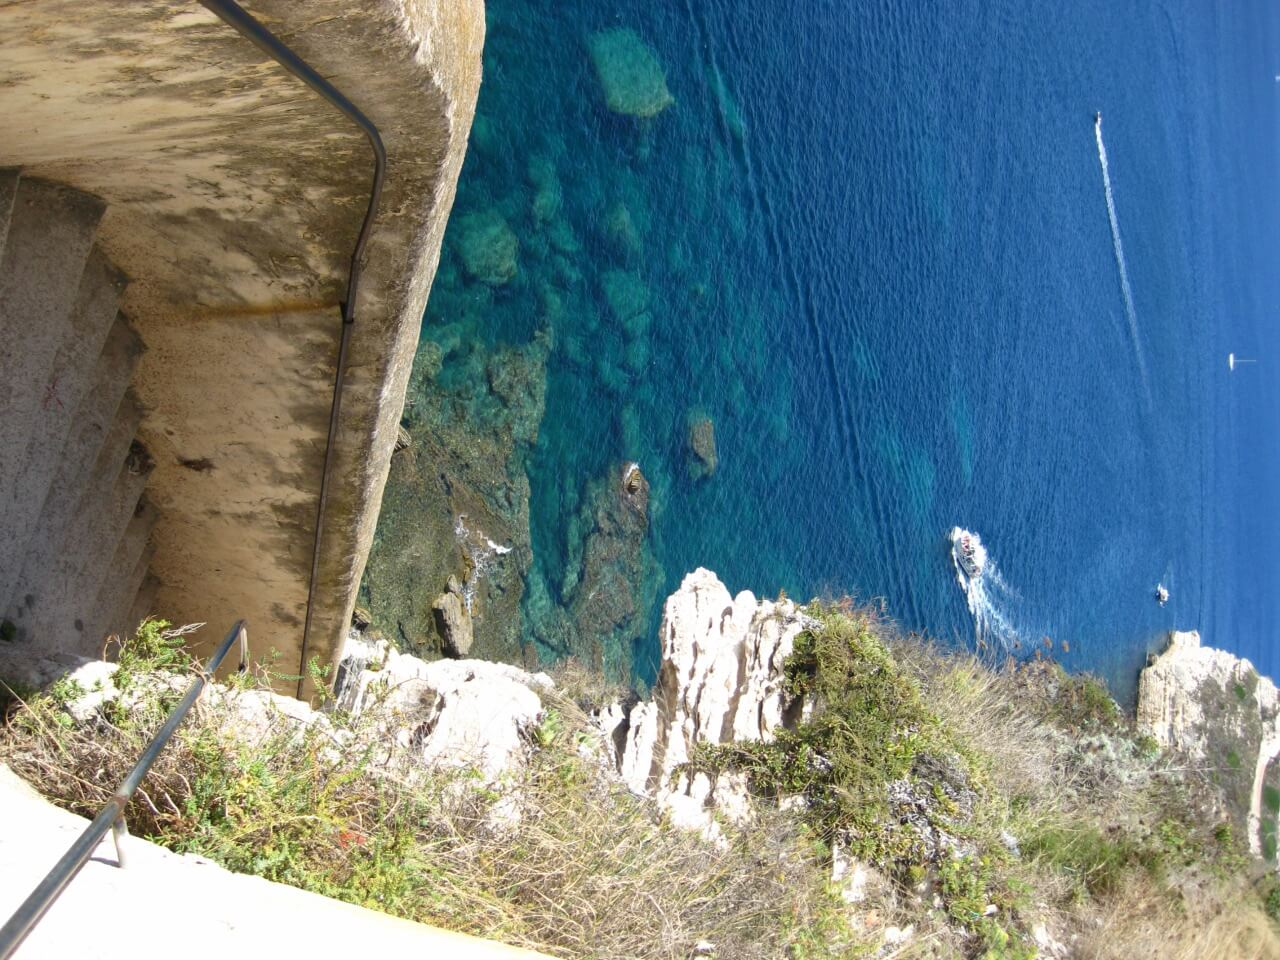
\includegraphics [width=0.3\textwidth]{../Bilder/Korsika/39.jpg}}\quad
   \subfloat{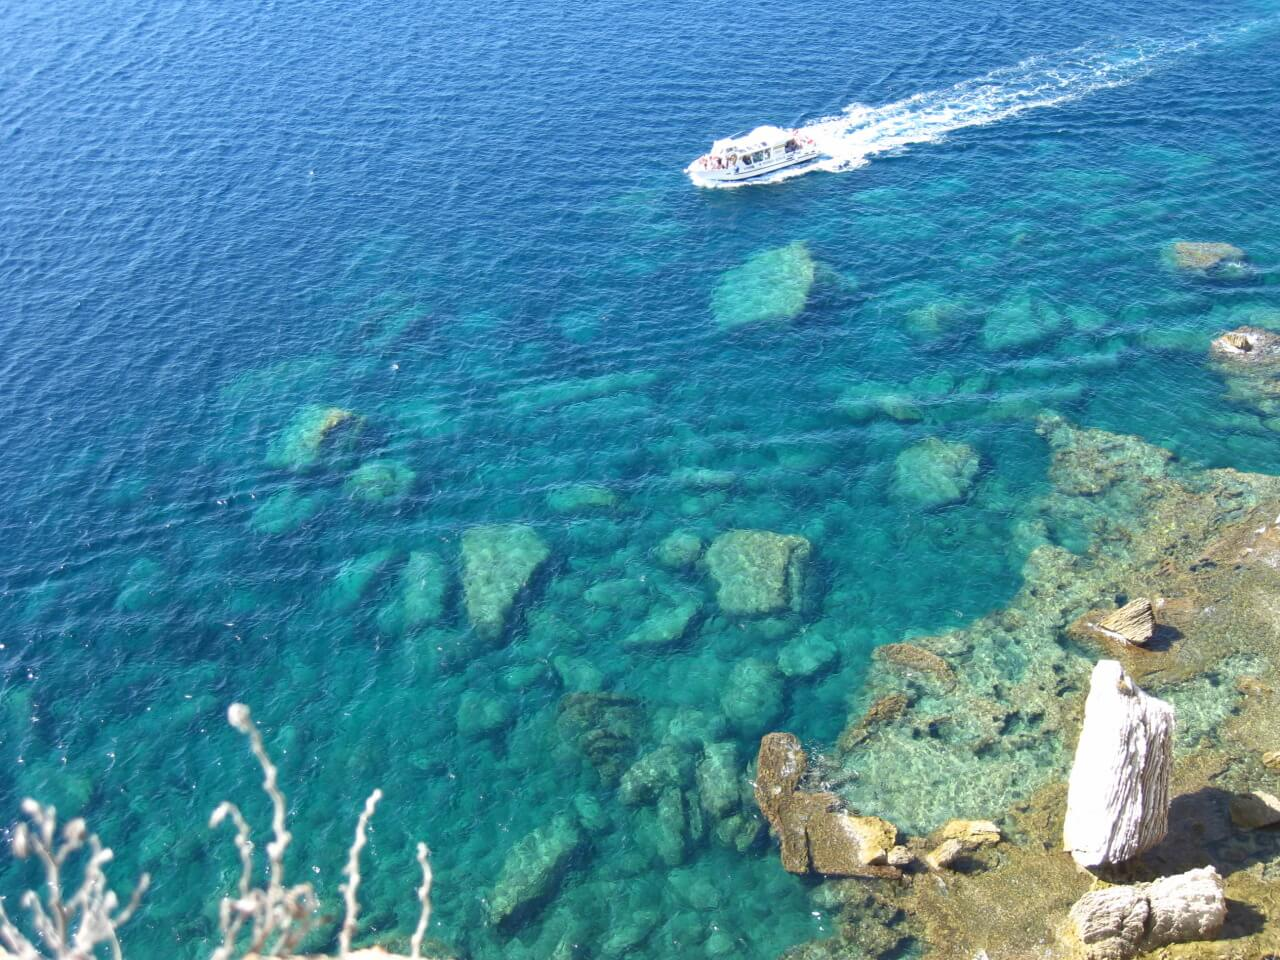
\includegraphics [width=0.3\textwidth]{../Bilder/Korsika/40.jpg}}\quad
   \subfloat{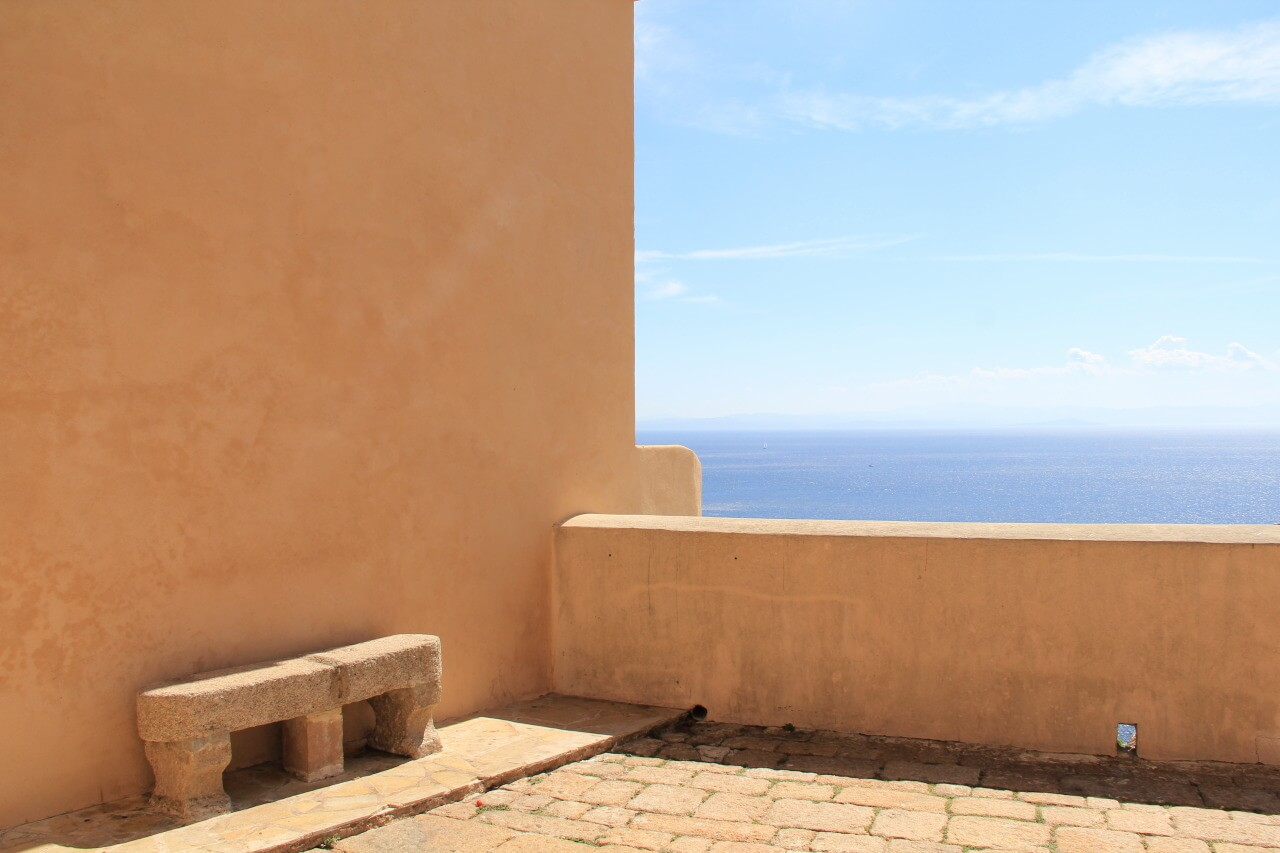
\includegraphics [width=0.3\textwidth]{../Bilder/Korsika/42.jpg}}\quad
   \caption[Idr�ck us Bonifacio]{Idr�ck us Bonifacio}
\end{figure}
Scho vor de 8tne semer h�t ufgstande, wells ade Rezeption gester vo de sehr fr�ndliche Dame gheisse het, wer nachem 8ti zum Beck gat (ein Ma chond jede Morge met sine Br�tli verbi), de chond norno Baguette �ber. So simer fasch Ponkt 8ti zum Becker unter de B�um und hend sogar na Croissant und Schoggi-Br�tli ergatteret. Hmm...fein sends gsi:) Nachem zMorge semer an Strand gh�cklet und send e das glasklare Wasser go schw�mme...esch wondersch�n und erfr�schend gsi. Zrugg ufem T�echli be ich scho gli ipfused und so eschs mer leider de ganz Tag gange...ich be entweder m�ed gsi, be en Trance gsi oder ha sosch chli umetr�umt...en richtigi Schlafm�tze be ich gsi. Aber mer hend trotzdem na es rechts Programm gmacht. Zersch semer es Zentrum vo Propriano go en Bankomat sueche. sSt�dtli esch recht touristisch, aber zemli herzig met de alte Granit-H�ser, de velle L�deli und G�ssli und em chline Hafe. De Bankomat esch zemli versteckt gsi, aber mer hend en schlussendlich doch na gfonde. Mer send de richtig Hafe glofe und hend em feine Duft vo de B�ckereie ned ch�ne widerstah. En Pizza, feini Zuckerb�lleli und e Glace hets ge:) Nach dem Snack simer zrugg zum Jack und witer nach Sartene, skorsiste St�dtli vo Korsika. D�t acho, hemer scho zemli schnell gmerkt, dass es wedermal sehr touristisch esch und mer fasch ke Parkplatz meh findet. Mer hend de doch na eine gfonde und send durs D�rfli gwagglet. Es het sch�ni, uralti und sehr engli G�ssli, aber esch fast zu touristisch, chli wie em Europapark. Nachere Fotisession semer de au scho witer uf Bonifacio, de s�dlichst Ponkt vo Korsika! Zersch hemer na enere Bucht welle go schnorchle oder surfe, aber mer hend nor sone komischi versnobbti, chli langwilligi Bucht gfonde, wo mer ned w�rkli het ch�ne go b�dele. So semer witerzottlet und hend scho gli das wondersch�ne uf Chridefelse baute Bonifacio erblickt. Da mer zersch uf euse Camping hend welle, send mer ade Stadt verbigfahre und send em Pfil Camping dIles gfolget....es esch ewigs gange bes mer denn endli bem Camping acho send. Em Reisef�hrer esch gstande mer cha met em Velo, evt. au zFuess ed Stadt laufe, aber da ch�mer also grad vergesse, es send �pe 8km uf Bonifacio, aber ufe und abe und vor allem ufe. Daher semer de grad do em Camping blebe und send met de Velo an relativ n�che Strand gradlet und send d�t na es St�ndli umeglege. Eigenli h�t die Bucht es Surferparadis s�lle si, aber vo Wind und Welle hemer ned so vell gmerkt. Nachem fulenze und s�nnele semer weder zu eusem Camping zrugd�set, go p�stele und hend zNacht kochet und zwar Ris met Chilli SENZA Carne. Da mer ned grad es mega Men� kochet hend, hemer denkt m�emer dev�r umso meh bem trinke investiere;) de t�rst Wi bes jetzt (14 Euro) hemer kauft, was dVerk�uferi em Lade fasch gschockt het..sie het gmeint: "Cest le plus cher...tu as vu.??"ouioui:) Leider esch er gar ned so fein gsi und ich ha weg mim Chopfweh gar ke Lust meh gha uf Wi. Dev�r ha ich vo mim Schatz e heissi Schoggi becho:) hmm esch super gsi! De Steff het nachli glese und ich be wie en Stei es Bettli plumpst und sofort ipfuused.

\subsection{11.09.2011 Sonntag}
\begin{wrapfigure}{R}{0.45\textwidth} 
  \begin{centering}
    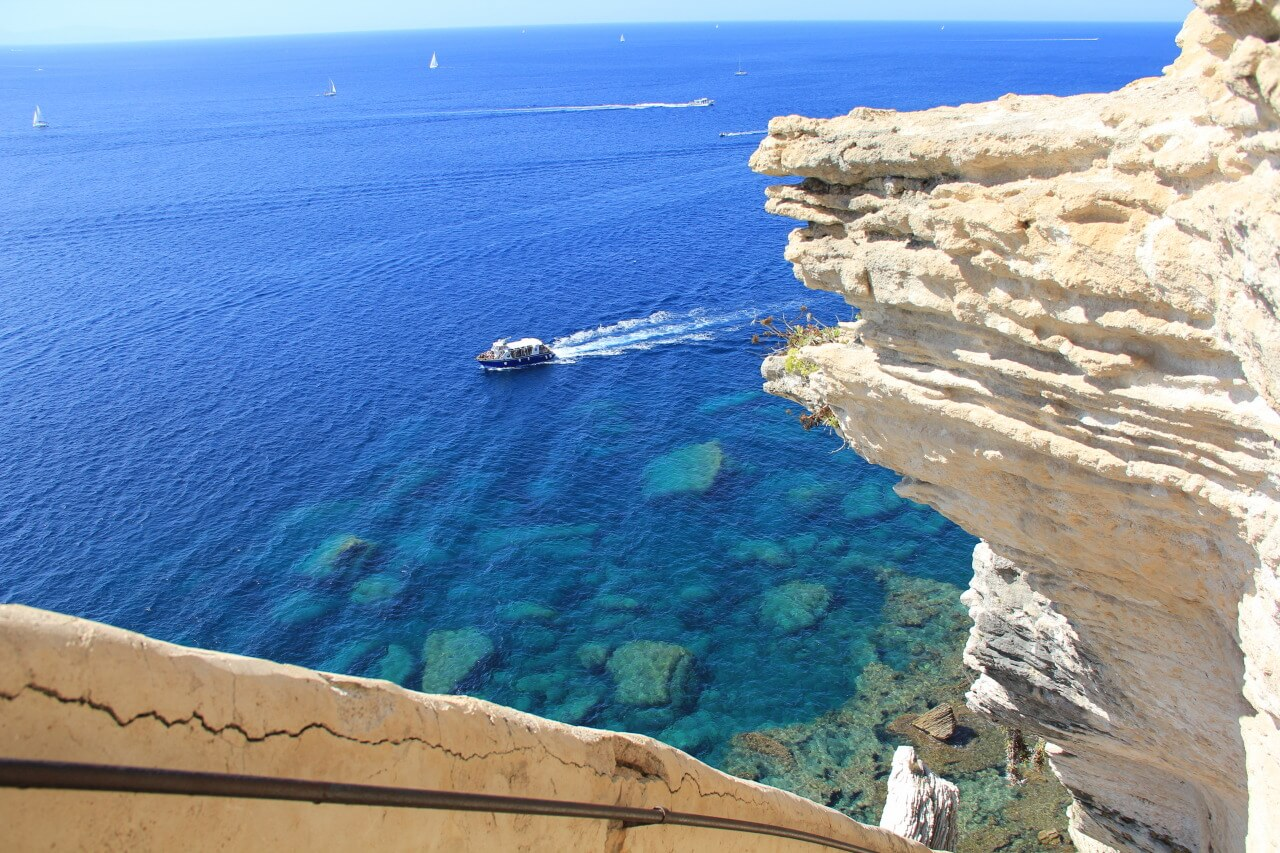
\includegraphics[width=0.4\textwidth, height=5cm, keepaspectratio]{../Bilder/Korsika/38.jpg}
    \caption{Bonifacio}
  \end{centering}
\end{wrapfigure} 
H�t hets feini Croissant und Schoggibr�tli zum zMorge ge. Gm�etlich hemers gno und send de um di 11i uf Bonifacio..wow die Stadt esch echt de Hammer! Zersch semer am Hafe umegschlenderet, wo de Steff ganz vell riiiiesigi Jachte bestunt het und fasch chli ifers�chtig worde esch. Neb de Schiff hets ganz vell Restaurants, Kaffis und Bars gha. De simer ufegwanderet ed Oberstadt vo Bonifacio,wos eus gfalle het und mer paar St�ndli verbrocht hend. Bonifacio esch uf steile, zum Teil �berh�ngende Chridefelse baut und daher sehr imposant. De Ufstieg ed Altstadt esch dementsprechend au zemli astrengend gsi, abere het sich uf all F�ll glohnt. Die ganz Oberstadt esch nemli voll vo herzigi G�ssli met vellne Restaurants, Souvenir-L�de und Kaffis. Zw�sched inne hesch na en super Ussecht vode Chridefelse abe uf das traumhafte-glasklare Meer. Zum Zmettag hemer e chli en grossi Thunpizza und feini Crevette gha:) Denn semer na uf de H�gel visavis vode Altstadt gloffe und hend vo d�t en geniali Ussecht uf dOberstadt unds Meer gha. Bem Abstieg ha ich fasch na es Herzchriesi becho, well churz vor mer en riiesige Schlange verbigschl�nglet esch...u���! De Steff het zersch n�t metbecho, well er sine Flugis nacheglueget het, ersch wo ich umegschroue und umegumpet be, het er sich gfragt, was e mich gfahre esch. Nach dem velle Umelaufe semer recht kaputti gsi und hend eus chli m�esse ufeme B�nkli erhole. Da aber ersch 4i gsi esch und mer na hend welle zNachtesse en Bonifacio, hemer na paar St�ndli vor eus gha. Darum hemer denkt: Mached mer doch na e chlini Bootstour:) Am 5i semer de met eme B�tli usem Hafe gfahre und send grad e di erscht Grotte inegfahre..wow..t�rkis-glasklars Wasser, Tropfstei und Chridefelse..het supersch� usgseh! De semer witer zode Lavazzi-Insle zo de Riche und Sch�ne und de weder zrug uf Bonifacio. Em sch�ne Obigsliecht het dAltstadt grandios usgseh und mer hend wedermal einigi F�teli gmacht. Mer het w�rkli sG�hl, die H�ser gheiet n�chstens grad es Wasser. Die steil Aragon-Treppe hemer vo witem au bestunt. Die semer am Mittag abeglofe und send fasziniert gsi vo de sch�ne Felse und dem traumhafte Wasser. Nor vom Ufstieg semer de n�m so begeisteret gsi;) dB�tlitour esch sehr erfr�schend gsi. Trotzdem semer zrug em Hafe enes Kaffi go en Ap�ro neh...uiuiui...mer eschs nacher zemli guet gange;) Min Moon-Drink het echli vell Prosecco denne gha, so dass ich grad es Glas umgschmisse ha. Leider esch em Steff sin Rucksack dusched worde. De semer enes Resti gschwankt;) und hend sehr fein zNachtgesse. Damol hets Seet�fel met Pfeffersauce und St.Pierre met N�ssli und Ris und Gm�es geh. Um di 10ni semer de zrug zo eusem Jack und uf de Campingplatz d�set. Esch en supersch�ne Tag gsi:)

\subsection{12.09.2011 Montag}
\begin{figure}[b]
   \centering
      %\subfloat[CAPTION]{BILDERCODE}\qquad
   \subfloat{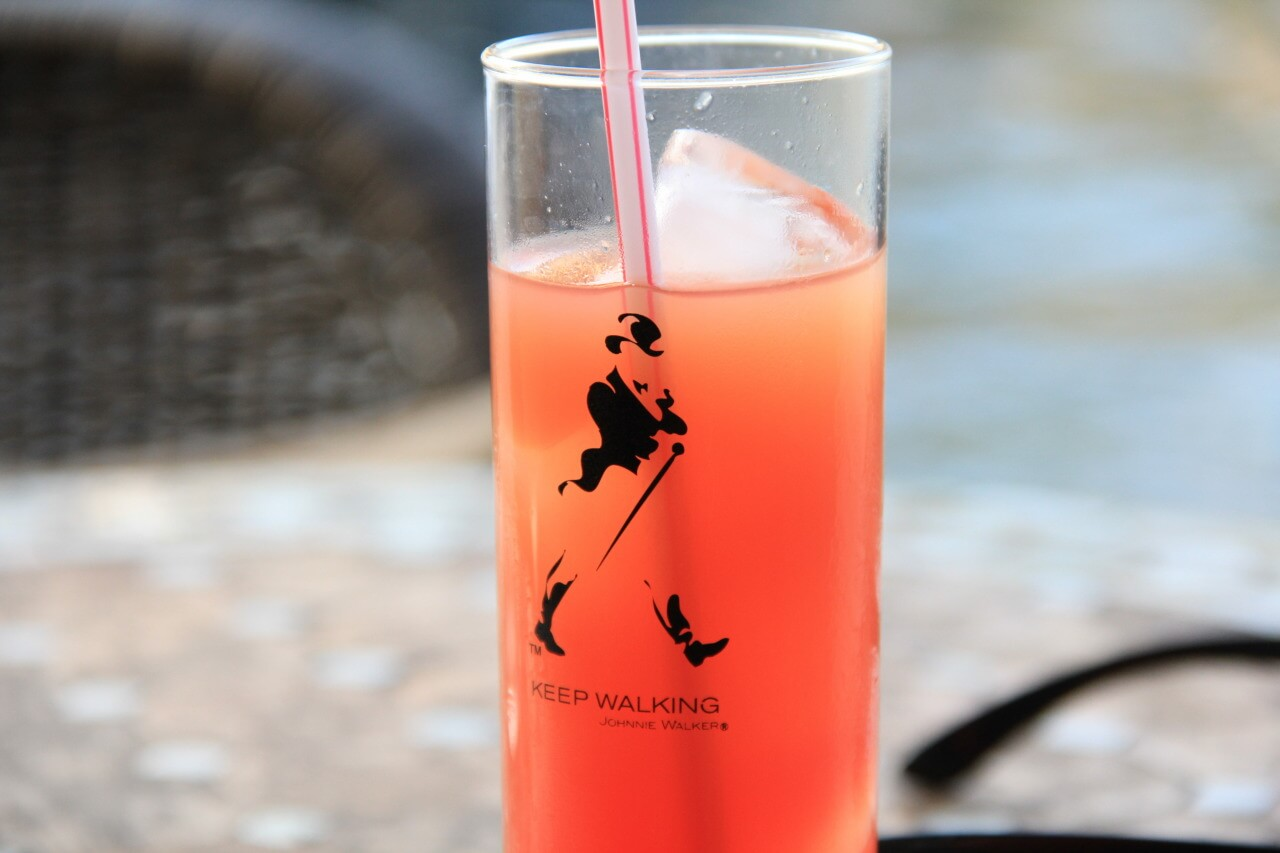
\includegraphics [width=0.3\textwidth]{../Bilder/Korsika/49.jpg}}\quad
   \subfloat{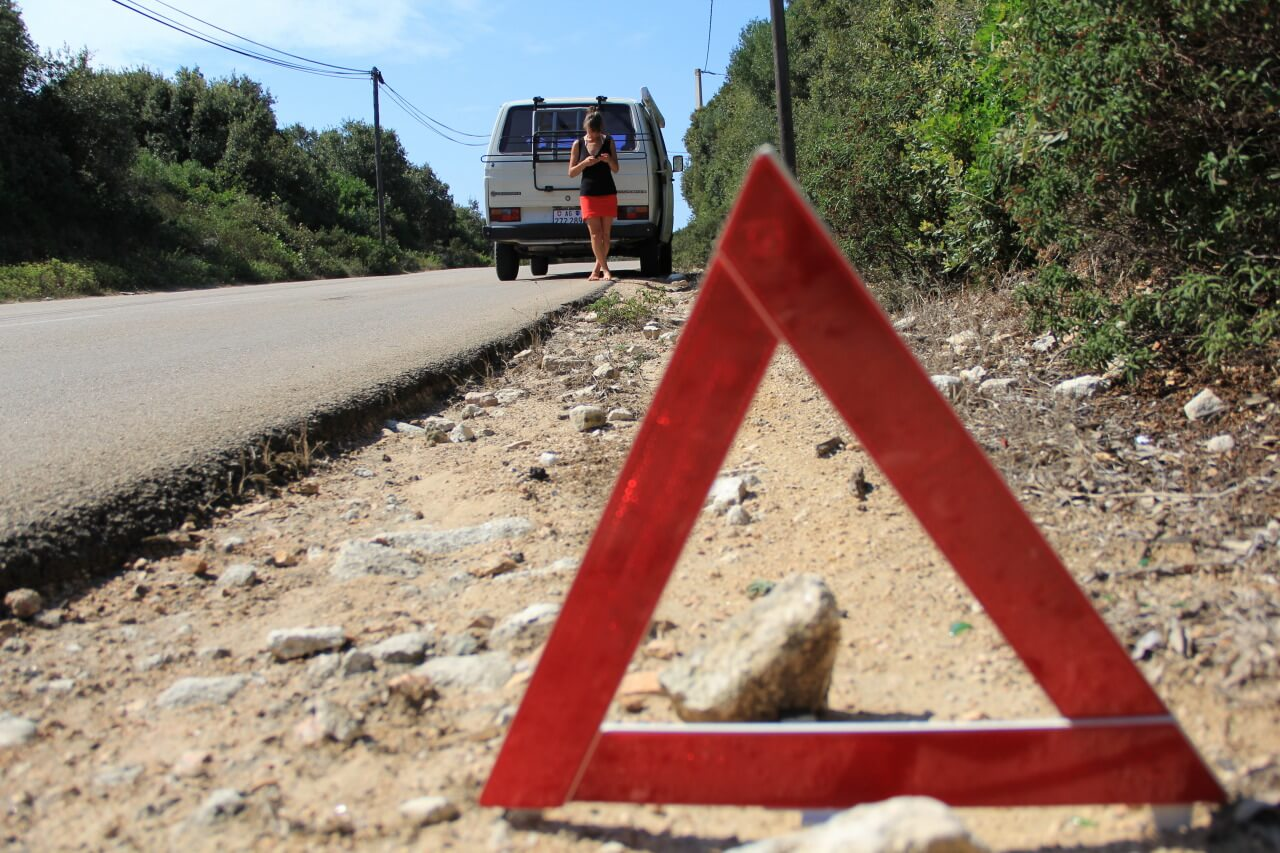
\includegraphics [width=0.3\textwidth]{../Bilder/Korsika/50.jpg}}\quad
   \subfloat{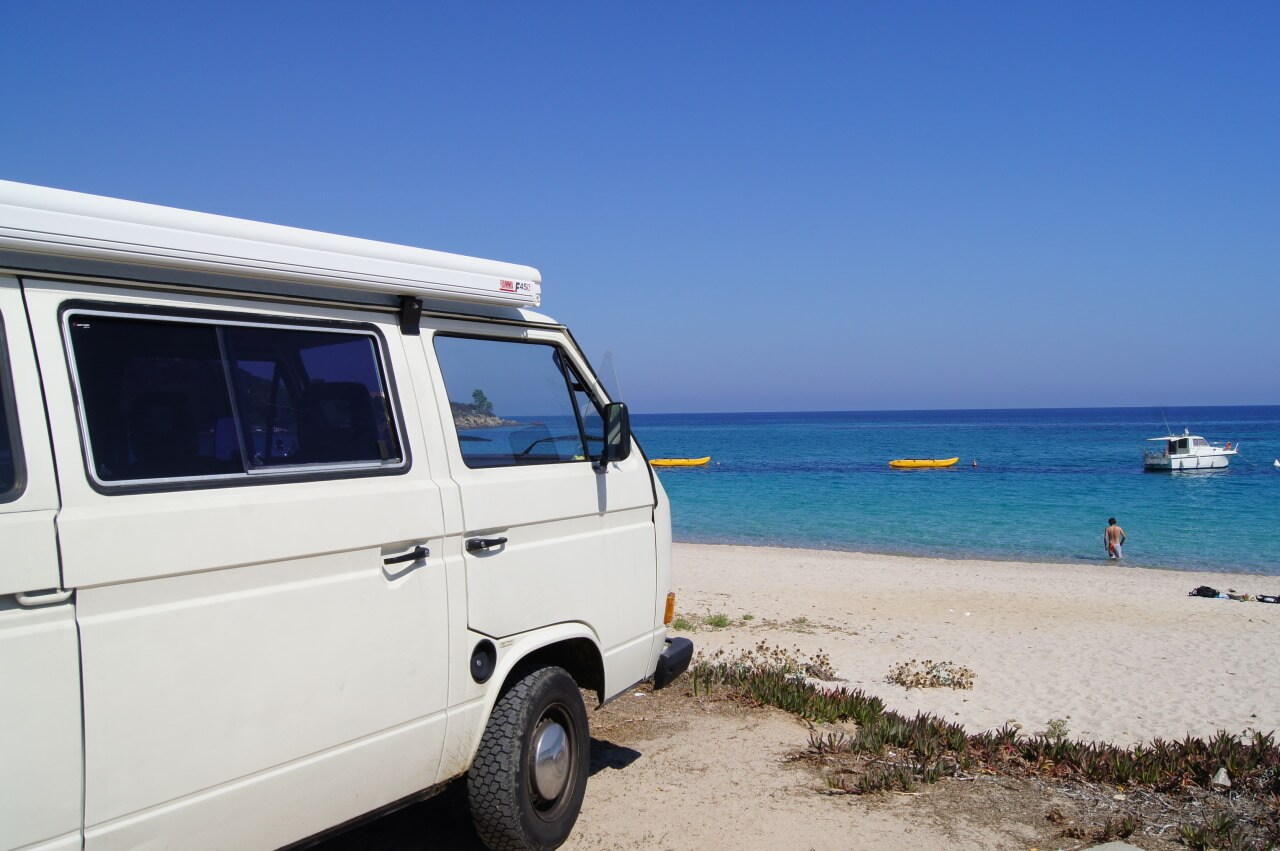
\includegraphics [width=0.3\textwidth]{../Bilder/Korsika/51.jpg}}\quad
   \caption[Pannentag]{Pannentag}
\end{figure}

Der Pechstag...fit und munter simer ufgstande,hend zm�rgelet und hend eus uf de Weg nach Bonifacio gmacht.
D�t hemer ghofft en schrubeziehr zfinde, um dKeilrieme vom jack ch�ne zflicke,da de so komischi Gr�sch vo sich get und internet, um mis Sprachmodul zBueche.
Beides hemer eigentli gschafft und trotzdem esch �pis ed Hose.
Ich ha am Hafe eme Internetkaffi ch�ne bueche und de Steff het zueff�llig en chline Werkz�glade gfonde.
Gl�cklich simer zrugg zu eusem Camping gfahre.
Ufem weg dethi hemer dKeilrieme na azoge und denkt;jetzt cha n�t meh schief ga;-) Leider hemer da falsch gedacht...
ufem Weg zo de supersch�ne Rondinarabucht,wo mer hend welle go b�dele, het euse Jack schlapp gmacht:-\ dKeilrieme send grisse und de Motor het gsprudlet..ohoh..
Das het ned guet usgseh.
Nachdem de Steff es paar mal probiert het die Rieme weder anezmache unds ned klappt het, hemer eusi Hoffnige ufgeh und hend em TCS agl�te.
Die hend gmeint: e einere Stond werdet er abgschleppet.
So hemer e eusem B�sli gwartet und gwartet.
De esch endli sAbschleppauto cho...
de Fahrer het ke Muks gseit,het de Jack ufglade und eus gfr�gt,�b mer wend metcho...
a klar hemer da welle,was h�ttet mer sosch s�lle mache? Wo mer gfr�get hend wos hi gat, het er gseit, nach porto veccio,d�t s�g di n�chst vw-garage.
Da simer grad chli verschrocke, da mer denkt hend mer g�nd enen Werkstatt en Bonifacio.
Aber Porto Veccio esch nor e halb Stond entfernt gsi.
Be de VW Garage acho, esch de Jack abglade worde und de Schleppwaage esch schoweder abd�set.
Mer send de inne go frage, wie lang dReperatur werd ga, da hend si nome gmeint; h�t werd er eh n�m aglueget, ersch morn morge und de meldet sie sich...
vorhe cha mer n�t s�ge.
Na super...so simer de H�gel ufe es Zentrum vo Porto Veccio zottlet und hend eus uf dSuechi vome Hotel gmacht.
Das esch gar ned so eifach gsi...
eis nachem andere h�mer abklapperet,aber leider n�t gfonde, alles esch complet gsi! Scho fasch hemer dHoffnig ufgeh und eus met em Gedanke vertraut gmacht am Strand zschlofe, als em letzte Hotel womer gfr�get hend, zwar au alles voll gsi esch, aber na es Abstellch�mmerli frei gsi esch.
Nat�rli hemer zuegseit und es esch gar ned so es chlises Zemmerli gsi.
Es het e Duschi, es WC(openair) und sogar en Fernseh gha.
Mer hend eus chic gmacht f�rs zNachtesse und send ed Altstadt vo Porto-Veccio.
St�dtli esch wondersch�n gsi met de velle chline,herzige und gm�etliche Restaurants,Kaffis und L�deli, wo sich ede enge G�ssli versteckt hend.
Znachtgesse hemer emene guete Resti ufere Terrasse, wo mer direkt uf de Hafe abe gseh het...wow...esch genial gsi!sEsse esch au himmlisch gsi! Mer hend grad es ganzes Men� gno: Rohschinke met Melone, Wildschweinlasagne, Penne met Lachs, Glace und �pfelchueche.
De Vollmond esch de na ufgange und es esch en wondersch�ne Obe gsi:-) Es het sich doch na zumene Gl�ckstag gwendet;-)

\subsection{13.09.2011 Dienstag}

\begin{wrapfigure}{R}{0.45\textwidth} 
  \begin{centering}
    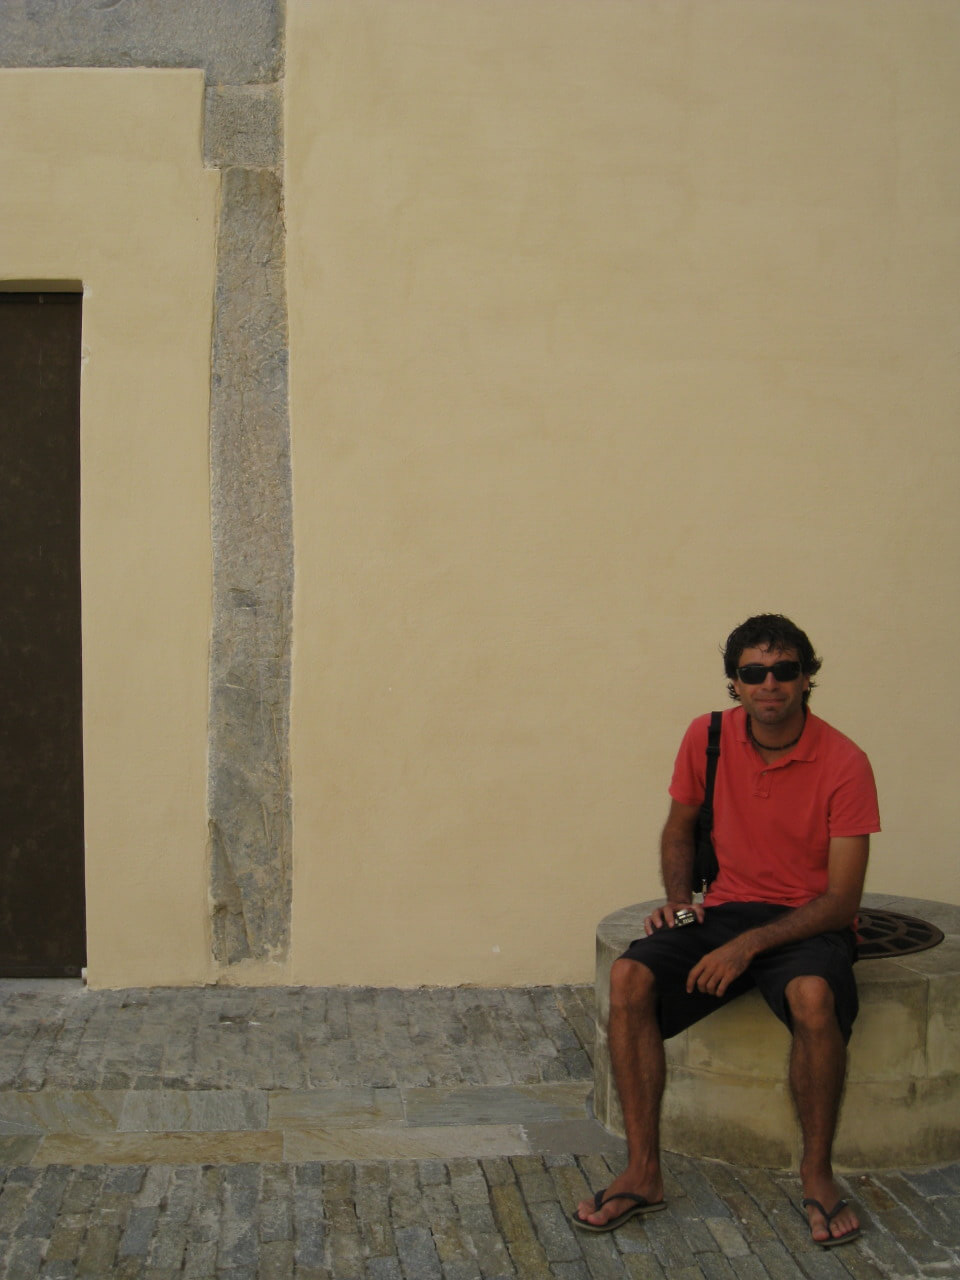
\includegraphics[width=0.4\textwidth, height=5cm, keepaspectratio]{../Bilder/Korsika/52.jpg}
    \caption{Ohni Bus unterwegs...}
  \end{centering}
\end{wrapfigure} 

Nachere vell zwarme Nacht und dementsprechend ned ganz so fit, simer uf de Garteterrasse vom Hotel fein go zm�rgele.
Gst�rkt simer ed VW Garage gloffe und hend ghofft, sie ch�nd eus scho meh Uskunft geh.
Aber wie erwartet esch na nix gange sie hend gseit, sie luegets am Namittag a...
uhh da ha ich schochli afo brodle und dampfe...
es het so t�nt,wie sie en am donnstig mal alueget und de mal lueget was zmache esch und keilrieme wahrschinli na m�end bstelle..grr..
mer hend de gseit, dass mer am Donnstig abreiset und so schnell wie m�glich s�tt gmacht werde.
Serschte wo mer jetzt hend welle, esch es Mietauto gsi, well mer emmerna eusi St�ehl, Tisch und Velos em Camping be Bonifaciogha hend und mer m�ed gsi send vom velle umelaufe.
So hemer em TCS agl�te, welli eus versicheret hen, dass sie eus es Mietauto organisieretund wo eus grad be de Garage abholt.
WOW..das esch na Service hemer denkt und send erliechteret noimet abgh�cklet und hend gwartet.
Nach �ber e Stond hemer eus langsam gfr�get, wo euses Auto esch, nach 2 Stond hemer namal agl�te.
De hets gheisse: ah ja ich ha ene grad welle al�te, sAuto staht parat bem Europcar! Jaja grad welle al�te, mer wartet 2 Stondund niemert informiert eus, echt en Frechheit! E dere Zyt h�ttet mer scho laang selber es Auto gmietet! Mer hend vermuetet, dass de Europcar bem Flughae esch und mer es Taxi m�end sueche. Da mer aber kes Taxi gfonde hend, semer enes Resti und hend d�t nach de Taxi-Telefonnummere gfr�get.
Zum Gl�ck het sie eus de gseit, dass Europcar grad um de Ecke esch, zum Gl�ck! Aber da de ersch weder am 2 ufgmacht het, hemer nachli Zit m�esse vertribe.
So simer nachli go shoppe:-) Mer send sogar erfolgrich gsi und es het neui Badhose, Hemdli und Flipflops geh.
Sauto hemer am 2 ch�ne abhole und so simer de au endli eusi verlorene Campingsache go hole.
Da mer eigentli scho laang hend welle go b�dele, simer de na gschnell an Strand gh�cklet.
Denn het de Steff e suuuper Nachricht becho: Euse Jack esch gflickt und abholbereit,jupiii! Schnell simer zode Garage d�set, hend de Jack gholt, sMietauto weder zruggeh und de sch�ni Camping Rondinara gfahre.
D�t hemer fein zNachtgesse(Tortellini) und send de gli go pfuse, da mer zemli m�ed gsi send.
Aber au sehr gl�cklich, well mer euse Jack weder gha hend:-)

\subsection{14.09.2011 Mittwoch}
Strandtag, jupiii :) H�t semer de gaaaaaaaanz Tag am wondersch�ne Rondinarastrand glege, hend gs�nnelet und b�delet.
sMeer esch glasklar und so sch�n t�rkis gsi, wie uf de Maledive.
Zum Bade esch es eifach traumhaft gsi.
Nebem ful umelege, hemer nachli Speedmington gspelt, was aber dank em Wind gar ned so eifach gsi esch.
Denn semer na go schnorchle.
De Steff esch extra am Mittag be gr�sster Hitz de steil Weg zum Camping ufegloffe und het eusi Schnorchelsache...
leider hets sich ned glohnt, well mer ussert paar chline Feschli und es paar Felse ned vell gseh het.
Dev�r hets sich glohnt, dass mer es Bodyboard kauft und mitgschleikt hend.
Wells ade Ostk�ste sooo hochi Welle gha het, hemer eus eher gf�hlt wie gstrandeti Wale als wie Surfer;-)
Zmettaggesse hemer em sch�ne Strandrestaurant.
Um di 6i semer zrug zo eusem Camping und hend euses zNacht vorbereitet, Ratatouille met Ris und feinem Ros�.
Nachem Esse hemer na �ber Gott und die Welt plauderet und send de ab es Bettli..
met emene chli warme, sonneuftankte Chopf.
Ou �pis hani na vergesse...
mer h�ttet eigentli super gschlafe, wenn euse liebi Nachbar, wo zersch e Liechtshow abzoge het, ned so lut gschnarchlet h�tt, dass de ganz Camping bebt h�tt und am Morge rings um en ume alli gfl�chtet send.

\subsection{15.09.2011 Donnerstag}
H�t heisst ab nach Bastia! Fr�e semer ufgstande und hend eus uf de Weg gmacht in Norde vo Korsika.
Zersch esch de Steff die voll krassi und kurverichigi Stross vom Camping zruggfahre und witer bis zume supersch�ne Sandstrand n�rdlich vo Porto Vecchio.
D�t semer zum letschte Mal namal e das wondersch�ne Meer gumpet und hends eifach gnosse.
Denn han ich denkt, jetzt cha ich witerfahre, send ja sch�ni, gradi und breiti Strasse...
esch au alles guet gange, bes mich es fetts Hummeli es F�dli gstoche het! Auuuua! Ich be ufgspronge, has St�rrad losglo, has Hummeli wegworfe und da hets mi grad namal en Finger gstoche! De Steff hets St�rrad m�esse �berneh, denn ha ich mich weder chli beruhigt und be uf dSite gfahre, usgstege und umegsprunge...haha..
de Steff het weder m�esse witerfahre und ich hami nebeddra versuechts erhole..
was gar ned so eifach gsi esch, wenn mer ned ufs F�dli cha hocke:-P
En Bastia acho, semer namal chli an Strand gh�cklet und send de es Zentrum an Hafe go zNachtesse.
Nachem Esse hemer na en Camping m�esse sueche und hend eus f�r de stadtn�chsti Platz entschede, wo ned w�rkli sch�n gsi esch, aber dev�r direkt am Meer.

\begin{figure}[H]
    \centering
    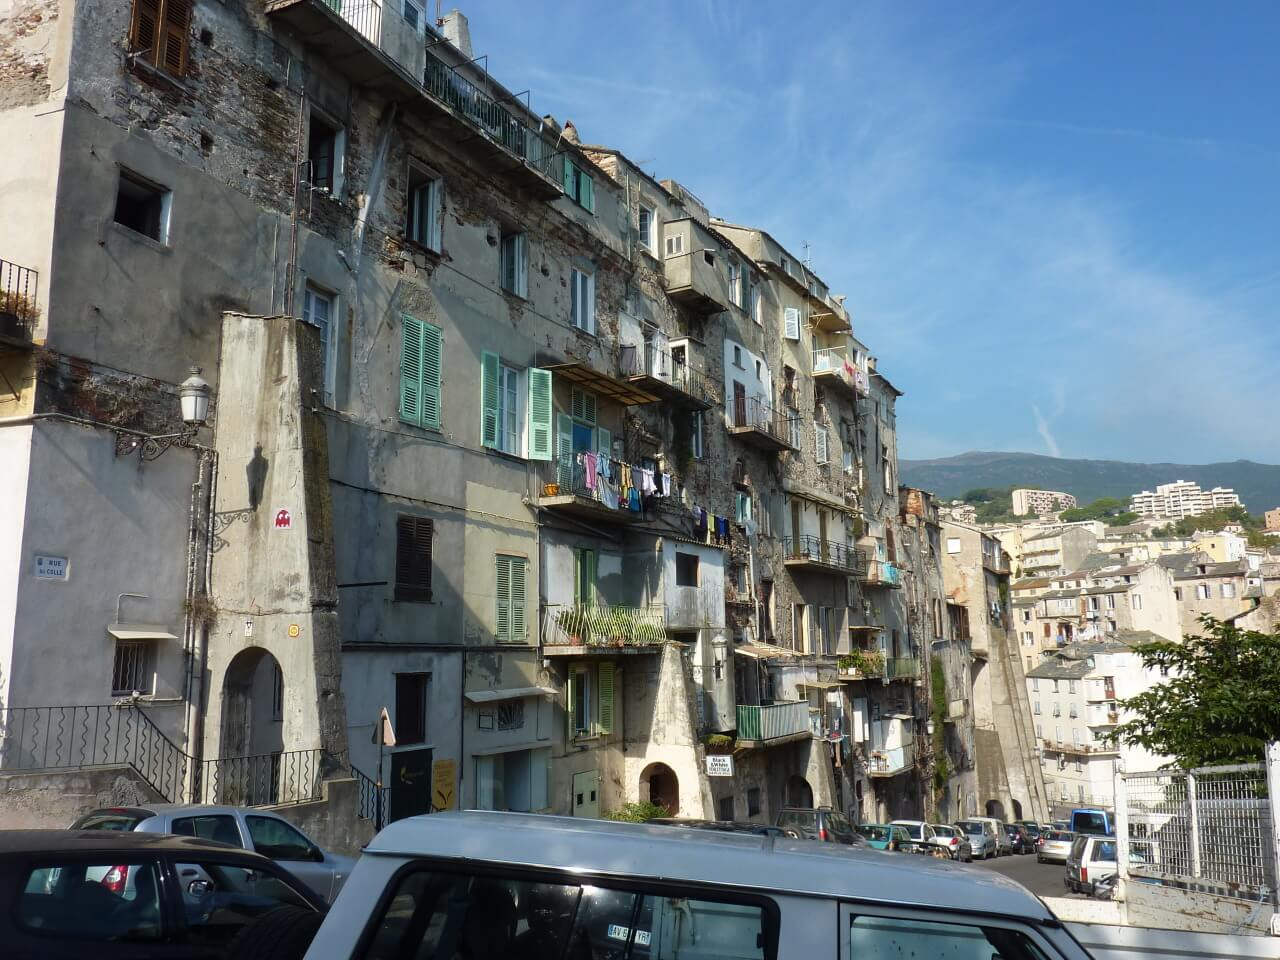
\includegraphics[width=\textwidth]{../Bilder/Korsika/53.jpg}
    \caption{Bastia}
    \label{img:Korsika3}
\end{figure}

\subsection{16.09.2011 Freitag}
H�t morge hemer die sch�ne sanit�re Anlage vo eusem super Campingplatz kenneglernt...
wu��� und de hends na neb eus sAbwasser abgloh.
Mer send de schnell uf Bastia innegfahre und hend ede sch�ne Altstadt zm�rgelet met wondersch�ne Ussecht uf de Hafe.
Mer send nachli ede Stadt umegschlenderet und hend de dF�hri ufgsuecht.
Die esch lang ned ume gsi, het sich de aber doch na blicke lo und de esch alles schnell gange.
Schlossendlich semer fascht rechtzitig abgfahre.
Mer hend euse Jack parkiert, send ufs Deck gst�rmt und hend na en Platz ergatteret zum s�nnele:) Die n�chste 5 Stond hemer met lese, s�nnele, Bricht schribe und esse verbracht;) En Genua acho, semer grad witergfahre durs Aostatal, wo mer fasch uf jedem H�gel sch�nbel�chteti Ruine gseh hend und dur de Gross Sankt Bernard, was 35 Franke kostet het.
Uf Sion het sichs de doch na lang zoge.
Ersch am halbi 2 semer en Sion acho und hend nebere Fabrik es �bernachtigspl�tzli gfonde.
M�ed vode lange Reis, aber gspannt uf dFlugshow morn, semer grad es Bett gheit und ipfused.

\begin{figure}[H]
    \centering
    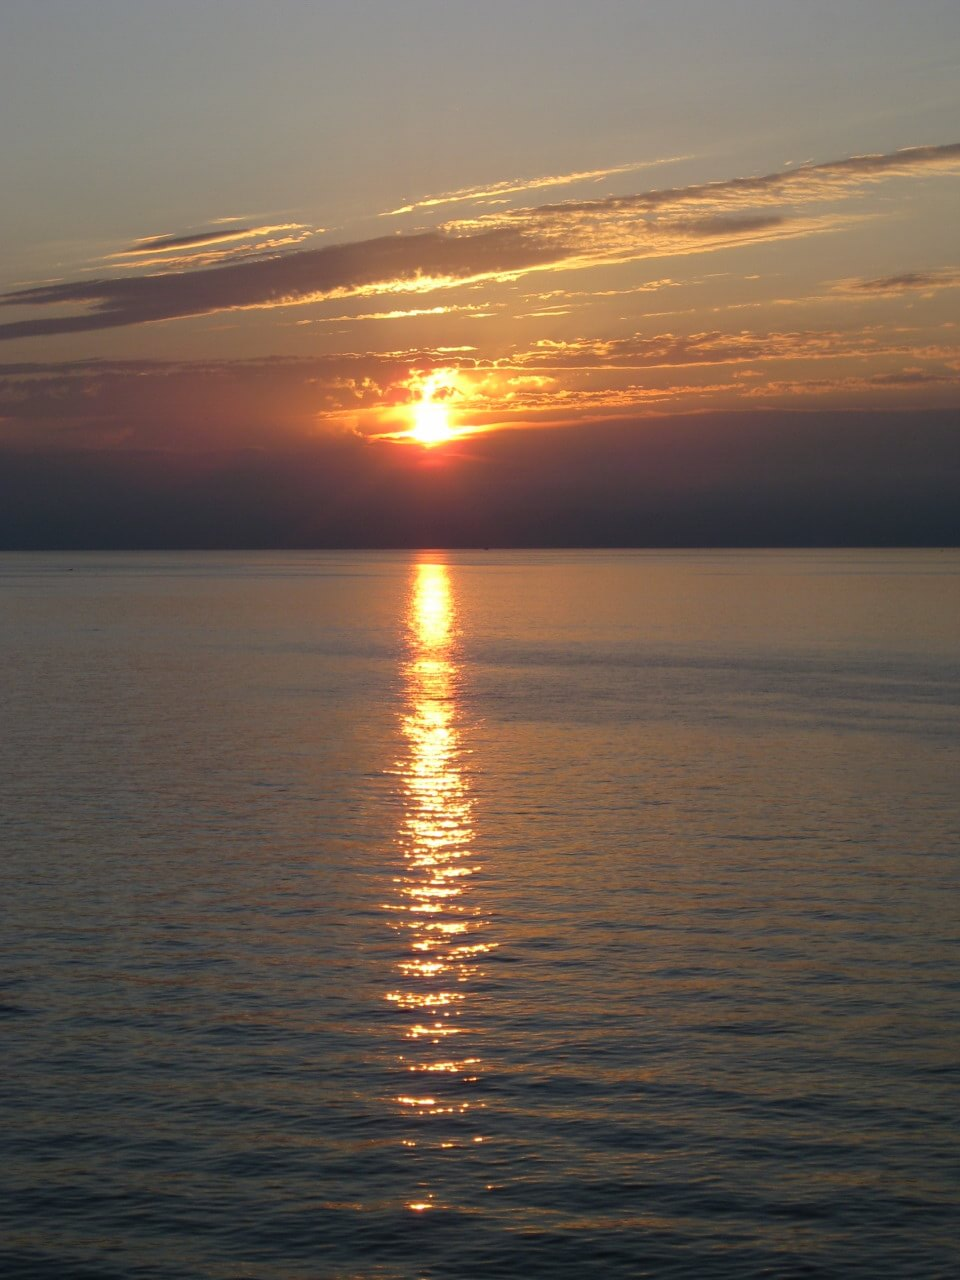
\includegraphics[width=\textwidth]{../Bilder/Korsika/54.jpg}
    \caption{Herrlichi Ferien gsi}
    \label{img:Korsika4}
\end{figure}

\newpage

\begin{figure}[H]
    \centering
    
\includegraphics[width=\textwidth,height=14cm, keepaspectratio]{../Bilder/Logo/Logo_trans.png}
    \label{img:Logo}
\end{figure}
\vfill
    \begin{center}
        {\huge  Weitere Informationen zum Bus und unseren Reisen sind auf der Homepage {\url{www.jackthebus.com}} zu finden}
\end{center}

\end{document}
